\documentclass[oneside]{book}

\input{./template/preamble}

\begin{document}
\include{./titlepage/titlepage}
%理论力学
%静力学公理和受力分析
%% ! TEX root = ../mechanics.tex 


\part{理论力学}

\chapter{静力学公理和受力分析}

\section{公理}
静力学一共由五条公理.
\begin{enumerate}
\item 力的平行四边形法则 \\
作用在物体上同一点的两个力,可以合成为一个合力,合力的作用点也在该点,
合力的大小和方向由这两个力为边构成的平行四边形法则的对角线确定,
\marginpar{制作插图}也就是合力矢等于这两个力矢的矢量和.
\item 二力平衡条件 \\
作用在同一刚体上的两个力,使刚体保持平衡的必要条件和充分条件是:这两个
力大小相等,方向相反,作用在同一直线上.三个条件缺一不可.
\item 加减平衡力系原理 \\
在任一原有力系上加上或减去任意的平衡力系,与原力系对刚体的作用效果
等效.由此可以得到两个推论.
\begin{enumerate}
\item 力的可传性 \\
作用在刚体上某点的力,可以沿着它的作用线移到刚体内的任意一点,并不改变
该力对刚体的作用.
\item 三力平衡汇交原理 \\
刚体在三个力的作用下平衡,若其中两个力的作用线交于一点,则第三个力的作用
线必通过此汇交点,且三个力位于同一个平面内.
\end{enumerate}
\item 作用和反作用定律 \\
作用力和反作用力总是同时存在, 两个力的大小总是大小相等,方向相反,沿着
同一条直线,分别作用在两个相互作用的物体上.
\begin{notice}
作用力和反作用力与二力平衡的区别在于,作用力和反作用
力作用在两个不同的物体上,而一对平衡力作用在同一个物体上.
\end{notice}
\item 刚化原理 \\
变形体在某一力系作用下处于平衡,如此将变形体刚化为刚体,其平衡状态保持不变.
\end{enumerate}

物体

%材料力学
%%! TEX root = ../mechanics.tex

\part{材料力学}

\chapter{基础知识}
\section{强度,刚度}
{\bfseries 强度}是衡量材料在不断裂的情况下可以承受应力
大小的量度,是材料在断裂或永久变形之前支撑最大载荷的能
力.

{\bfseries 刚度}是衡量材料受到外力作用变形后恢复原状的
能力,是指材料抵抗外力仍能恢复原状的能力.

强度可以划分为
\begin{equation*}
  \color{titleblue}
  \begin{cases}
    抗拉强度\\
    冲击强度\\ 
    抗压强度\\ 
    屈服强度和极限强度
  \end{cases} 
\end{equation*}


%空气动力学
%基本知识介绍
\include{./aerodynamics/introductory_thoughts}
%场论
\include{./aerodynamics/Field_theory_review}
%基本方程
\include{./aerodynamics/fundamental_equations}
%不可压无粘流
\include{./aerodynamics/incompressible_inviscous_flow}
%高速可压流动
\include{./aerodynamics/high-speed_pressure_flow}
%低速翼型气动特性
\include{./aerodynamics/Incompressible_Flow_over_Airfoils}
%火箭导弹技术引论
%导弹概论
% % ! TEX root = ../mechanics.tex
%火箭导弹概论

\part{火箭导弹技术引论}
\chapter{概述}
\section{火箭弹的特点}
相较于身管武器(火炮),火箭弹武器系统的特点是:
\begin{enumerate}
	\item 有较高的飞行速度
	\item 发射时无后座力
	\item 发射时的过载系数小
\end{enumerate}
缺点是:
\begin{enumerate}
	\item 密集度较差
	\item 容易暴露发射阵地
	\item 造价比相同威力的炮弹高
\end{enumerate}

\section{火箭导弹的分类}
按照稳定方式分类的火箭弹
\begin{equation*}
	\color{titleblue}
	\begin{cases}
		 \text{尾翼稳定火箭弹} \\
		 \text{旋转稳定火箭弹}
	\end{cases}
\end{equation*}
\begin{notice}
	\begin{itemize}
		\item 尾翼稳定火箭弹的特点:\\
		      弹身较长,装药量大,射程远,
		      抗干扰能力高,稳定性高.
		\item 旋转稳定火箭弹的特点:\\
		      火箭弹高速旋转,能减少推力偏心和
          质量偏心的不良影响,提高
		      密集度;弹身较短,没有尾翼,
          易于实现机械化装填但弹长
          受限,难以增加发动机装药量.
	\end{itemize}
\end{notice}


按照用途方式分类的火箭弹
\begin{equation*}
	\color{titleblue}
	\begin{cases}
		 \text{反坦克火箭弹} \\
		 \text{野战火箭弹}  \\
		 \text{航空火箭弹}
	\end{cases}
\end{equation*}

\section{火箭弹的战术技术要求}
\begin{equation*}
	\color{titleblue}
	\begin{cases}
		 \text{射程}    \\
		 \text{威力}    \\
		 \text{密集度}   \\
		 \text{机动性}   \\
		 \text{安全可靠性}
	\end{cases}
\end{equation*}

\section{导弹}
按照射程可以分为
\begin{equation*}
	\color{titleblue}
	\begin{cases}
		 \text{近程导弹} \\
		 \text{中程导弹} \\
		 \text{远程导弹} \\
		 \text{洲际导弹}
	\end{cases}
\end{equation*}

\begin{equation*}
	\color{titleblue}
	\begin{cases}
		 \text{面对面导弹}   \\
		 \text{面对空导弹}   \\
		 \text{空对面导弹}   \\
		 \text{空对空导弹}   \\
		 \text{反舰(潜)导弹} \\
		 \text{反坦克导弹}
	\end{cases}
\end{equation*}

\subsection{组成部分}
\begin{equation*}
	\color{titleblue}
	\begin{cases}
		 \text{动力装置:为导弹提供飞行动力}       \\
		 \text{制导系统:将导弹导向目标}         \\
		 \text{战斗部:直接毁伤目标,完成战斗任务的部分} \\
		 \text{弹体:以安装战斗部,控制系统,动力装置,
		推进剂和弹上电源等}                     \\
		 \text{给弹上各分系统工作用电的电能装置}
	\end{cases}
\end{equation*}

\subsection{导弹战斗技术指标}
\begin{equation*}
	\color{titleblue}
	\begin{cases}
		 \text{战术要求}
		\begin{cases}
			 \text{导弹类别}  \\
			 \text{战斗部威力} \\
			 \text{命中概率}  \\
			 \text{飞行性能}
		\end{cases}     \\
		 \text{技术要求}
		\begin{cases}
			 \text{发动机类别}     \\
			 \text{导弹极限尺寸和重量} \\
			 \text{所用材料限制}
		\end{cases} \\
		 \text{使用维护要求}
		\begin{cases}
			 \text{部件互换性}     \\
			 \text{运输方便}      \\
			 \text{操作安全,贮存期限}
		\end{cases}
	\end{cases}
\end{equation*}


%导弹飞行原理
% % ! TEX root = ../mechanics.tex

%导弹飞行原理
\chapter{火箭导弹飞行原理}
\section{总空气动力}
\subsection{地面坐标系$Oxyz $}
发射点为原点$O$,弹道面与水平面
的交线为$Ox$轴,$Oy$轴在包含$Ox$的
铅锤面内,与$Ox$轴垂直,$Oz$轴按
右手螺旋法则确定.
\subsection{弹道坐标系$Ox_2y_2z_2$}
弹体质心为原点$O$,$Ox_2$轴与弹体质心
的速度矢量重合,$Oy_2$在包含$Ox_2$轴的
铅锤面内,并且与$Ox_2$垂直,$Oz_2$轴按
右手螺旋法则确定.
\subsection{速度坐标系$Ox_3y_3z_3$}
原点$O$在弹体的质心上,$Ox_3$轴与速度
矢量重合,$Oy_3$位于弹体纵向对称面内,
并与$Ox_3$垂直,$Oz_3$垂直于$Ox_3y_3$
平面,按右手螺旋法则确定方向.
\subsection{弹体坐标系$Ox_1y_1z_1$}
原点$O$取在弹体质心上,$Ox_1$与弹体
纵轴垂直,指向头部为正,$Oy_1$轴在弹体
纵向对称面内,垂直$Ox_1$轴,指向上方为正,
$Oz_1$垂直$Ox_1y_1$平面,按右手螺旋法则
确定方向.

两个坐标系都是动坐标系.

\begin{notice}
	\begin{enumerate}
		\item {\bfseries 攻角}\index{攻角}$\alpha$ \\
		      速度矢量$\mathbf{V}$在纵向对称平面
		      $Ox_1y_1$上的投影和$Ox_1$的夹角,若
		      $Ox_1$轴位于投影线的上方,则攻角$\alpha$
		      为正.
		\item {\bfseries 侧滑角}\index{侧滑角}$\beta$ \\
		      速度矢量$\mathbf{V}$在纵向对称平面$Ox_1y_1$
		      之间的夹角.若来流从右侧流向弹体则为正.(从
		      飞行方向观察)
        \item {\bfseries 俯仰角}\index{俯仰角}$\Xi$\\ 
          弹体纵轴$Ox_1$与水平面的夹角.
        \item {\bfseries 偏航角}\index{偏航角}$\Psi$\\ 
          弹体纵轴$Ox_1$在水平面内的投影与$Ox$的夹角.
        \item {\bfseries 滚转角}\index{滚转角}$\gamma$\\ 
          弹体坐标系$Oy_1$轴与包含弹体纵轴铅锤平面的夹角.
        \item {\bfseries 弹道倾角}\index{弹道倾角}$\theta$\\ 
          速度矢量$\mathbf{V}$与水平面的夹角.
        \item {\bfseries 弹道偏角}\index{弹道偏角}$\Psi_v$\\ 
          速度矢量$\mathbf{V}$在水平面内的投影与$Ox$的夹角.
        \item {\bfseries 速度倾斜角}\index{速度倾斜角}$\gamma_v$\\ 
          $Oy_3$与包含速度矢量$\mathbf{V}$的铅锤面的夹角.
	\end{enumerate}
	%tikz
	% ! TEX root = ./principle_of_flight.tex

\begin{center}

\tikzset{every picture/.style={line width=0.75pt}} %set default line width to 0.75pt        

\begin{tikzpicture}[x=0.75pt,y=0.75pt,yscale=-1,xscale=1]
%uncomment if require: \path (0,300); %set diagram left start at 0, and has height of 300

%Shape: Rectangle [id:dp1411189406840021] 
\draw  [fill={rgb, 255:red, 245; green, 166; blue, 35 }  ,fill opacity=1 ] (161.6,153.7) -- (392.24,99) -- (401.53,137.64) -- (170.89,192.34) -- cycle ;
%Straight Lines [id:da2938932926787814] 
\draw [color={rgb, 255:red, 74; green, 144; blue, 226 }  ,draw opacity=1 ]   (313.35,237.9) -- (265.85,51.2) ;
\draw [shift={(265.35,49.27)}, rotate = 75.72] [color={rgb, 255:red, 74; green, 144; blue, 226 }  ,draw opacity=1 ][line width=0.75]    (10.93,-3.29) .. controls (6.95,-1.4) and (3.31,-0.3) .. (0,0) .. controls (3.31,0.3) and (6.95,1.4) .. (10.93,3.29)   ;
%Straight Lines [id:da07973104503934425] 
\draw [color={rgb, 255:red, 126; green, 211; blue, 33 }  ,draw opacity=1 ]   (289.35,143.58) -- (361.8,85.27) ;
\draw [shift={(363.35,84.01)}, rotate = 141.17] [color={rgb, 255:red, 126; green, 211; blue, 33 }  ,draw opacity=1 ][line width=0.75]    (10.93,-3.29) .. controls (6.95,-1.4) and (3.31,-0.3) .. (0,0) .. controls (3.31,0.3) and (6.95,1.4) .. (10.93,3.29)   ;
%Straight Lines [id:da5051642498138564] 
\draw [color={rgb, 255:red, 126; green, 211; blue, 33 }  ,draw opacity=1 ]   (289.35,143.58) -- (225.65,68.66) ;
\draw [shift={(224.35,67.14)}, rotate = 49.63] [color={rgb, 255:red, 126; green, 211; blue, 33 }  ,draw opacity=1 ][line width=0.75]    (10.93,-3.29) .. controls (6.95,-1.4) and (3.31,-0.3) .. (0,0) .. controls (3.31,0.3) and (6.95,1.4) .. (10.93,3.29)   ;
%Straight Lines [id:da16788098204645885] 
\draw [color={rgb, 255:red, 126; green, 211; blue, 33 }  ,draw opacity=1 ]   (289.35,143.58) -- (374.69,200.06) ;
\draw [shift={(376.35,201.16)}, rotate = 213.5] [color={rgb, 255:red, 126; green, 211; blue, 33 }  ,draw opacity=1 ][line width=0.75]    (10.93,-3.29) .. controls (6.95,-1.4) and (3.31,-0.3) .. (0,0) .. controls (3.31,0.3) and (6.95,1.4) .. (10.93,3.29)   ;
%Straight Lines [id:da8889478781385203] 
\draw [color={rgb, 255:red, 74; green, 144; blue, 226 }  ,draw opacity=1 ]   (289.35,143.58) -- (256.08,229.08) ;
\draw [shift={(255.35,230.95)}, rotate = 291.26] [color={rgb, 255:red, 74; green, 144; blue, 226 }  ,draw opacity=1 ][line width=0.75]    (10.93,-3.29) .. controls (6.95,-1.4) and (3.31,-0.3) .. (0,0) .. controls (3.31,0.3) and (6.95,1.4) .. (10.93,3.29)   ;
%Straight Lines [id:da9590319678742609] 
\draw [color={rgb, 255:red, 74; green, 144; blue, 226 }  ,draw opacity=1 ]   (289.35,143.58) -- (373.85,102.55) ;
\draw [shift={(375.65,101.68)}, rotate = 154.1] [color={rgb, 255:red, 74; green, 144; blue, 226 }  ,draw opacity=1 ][line width=0.75]    (10.93,-3.29) .. controls (6.95,-1.4) and (3.31,-0.3) .. (0,0) .. controls (3.31,0.3) and (6.95,1.4) .. (10.93,3.29)   ;
%Straight Lines [id:da8595472323255129] 
\draw [color={rgb, 255:red, 208; green, 2; blue, 27 }  ,draw opacity=1 ]   (363.35,84.01) -- (375.65,101.68) ;
%Curve Lines [id:da30781488459018513] 
\draw    (332.5,122.63) .. controls (338.65,120.54) and (342.65,132.45) .. (334.65,133.44) ;
%Curve Lines [id:da3508432857182251] 
\draw    (326.35,113.8) .. controls (332.65,107.63) and (338.65,116.57) .. (332.5,122.63) ;
%Straight Lines [id:da500424813028004] 
\draw [color={rgb, 255:red, 80; green, 227; blue, 194 }  ,draw opacity=1 ]   (167.65,133.44) -- (207.88,154.36) ;
\draw [shift={(209.65,155.29)}, rotate = 207.48] [color={rgb, 255:red, 80; green, 227; blue, 194 }  ,draw opacity=1 ][line width=0.75]    (10.93,-3.29) .. controls (6.95,-1.4) and (3.31,-0.3) .. (0,0) .. controls (3.31,0.3) and (6.95,1.4) .. (10.93,3.29)   ;
%Shape: Triangle [id:dp056219082178769586] 
\draw  [fill={rgb, 255:red, 245; green, 166; blue, 35 }  ,fill opacity=1 ] (526.49,88.87) -- (401.53,137.64) -- (392.46,98.97) -- cycle ;
%Straight Lines [id:da07013554849919856] 
\draw [color={rgb, 255:red, 74; green, 144; blue, 226 }  ,draw opacity=1 ]   (87.15,191.44) -- (580.21,75.9) ;
\draw [shift={(582.15,75.44)}, rotate = 166.81] [color={rgb, 255:red, 74; green, 144; blue, 226 }  ,draw opacity=1 ][line width=0.75]    (10.93,-3.29) .. controls (6.95,-1.4) and (3.31,-0.3) .. (0,0) .. controls (3.31,0.3) and (6.95,1.4) .. (10.93,3.29)   ;

% Text Node
\draw (344.33,72.13) node [anchor=north west][inner sep=0.75pt]    {$\mathbf{V}$};
% Text Node
\draw (264.33,130.79) node [anchor=north west][inner sep=0.75pt]    {$O$};
% Text Node
\draw (560,79.32) node [anchor=north west][inner sep=0.75pt]    {$x_{1}$};
% Text Node
\draw (370,72.54) node [anchor=north west][inner sep=0.75pt]    {$x_{3}$};
% Text Node
\draw (274,47.04) node [anchor=north west][inner sep=0.75pt]    {$y_{1}$};
% Text Node
\draw (216.67,73.86) node [anchor=north west][inner sep=0.75pt]    {$y_{3}$};
% Text Node
\draw (247,198.59) node [anchor=north west][inner sep=0.75pt]    {$z_{1}$};
% Text Node
\draw (356,195.64) node [anchor=north west][inner sep=0.75pt]    {$z_{3}$};
% Text Node
\draw (345.33,112.59) node [anchor=north west][inner sep=0.75pt]    {$\alpha $};
% Text Node
\draw (345.67,91.71) node [anchor=north west][inner sep=0.75pt]    {$\beta $};
% Text Node
\draw (129,115.82) node [anchor=north west][inner sep=0.75pt]   [align=left] {纵向对称面};


\end{tikzpicture}
\end{center}

\end{notice}
\subsection{总空气动力}
{\bfseries 总空气动力}\index{总空气动力}可以
沿速度坐标系分解为升力$Y$,
阻力$X$,侧向力$Z$.
\begin{equation*}
	\begin{split}
		X&=C_x q S \\
		Y&=C_y q S \\
		Z&=C_z q S
	\end{split}
\end{equation*}
其中$q$是动压,$q=\frac{1}{2}\rho V^2$,
$S$是火箭的特征面积.$C_x$,$C_y$,$C_z$分别是
阻力系数,升力系数和侧向力系数.
\begin{note}
	空气动力的大小与来流的动压$q$和火箭的特征面积
	$S$成正比.
\end{note}
\begin{notice}
	\begin{enumerate}
		\item {\bfseries 升力}\index{升力} \\
		      全弹的升力可以看成是弹翼,弹身,尾翼(舵面)等
		      各部件产生的升力之和加上各部件之间相互干扰
		      的附加升力.弹翼是提供升力的主要部件,其余产
		      生的升力很小.

          升力系数基本上是马赫数,攻角,升降舵的舵面偏角的函数.
		      \begin{note}
			      升力系数大小与攻角有关,在一定范围内,攻角越大,升
			      力系数越大,超过之后,攻角再增大,升力系数急剧
			      减小,飞机失速.
		      \end{note}
        \item {\bfseries 侧向力}\index{侧向力}\\ 
          侧向力系数基本上取决于马赫数,侧滑角,
          方向舵舵面偏转角.
		\item {\bfseries 阻力}\index{阻力} \\
		      作用在火箭导弹上的总空气动力在速度方向上的分量
		      就是阻力,它总是与速度方向相反,起到阻碍火箭导弹
		      运动的作用.
		      \begin{note}
			      阻力受空气的粘性影响最为显著.
		      \end{note}
		      导弹的空气阻力通常被分为两部分.
		      \begin{enumerate}
			      \item {\bfseries 零升阻力}\\
			            升力为零时的阻力.分为摩擦阻力和压差阻力.
			      \item {\bfseries 诱导阻力}\\
			            由升力或侧向力诱导出来的阻力(即与升力或者
			            侧向力大小有关).
		      \end{enumerate}
          诱导阻力是伴随升力而产生的,没有升力也就没有诱导阻力.
	\end{enumerate}
\end{notice}

\section{总空气力矩}
将总空气力矩沿弹体坐标系分解为三个分量,分别为
滚转力矩$M_x$,偏航力矩$M_y$,俯仰力矩$M_z$,气动
力矩的表达式为
\begin{equation*}
  \begin{split}
    M_x&=m_x q S L\\ 
    M_y&=m_y q SL \\ 
    M_z&=m_z q SL 
  \end{split}
\end{equation*}
其中,$m_x $,$m_y $,$m_z $
分别是滚转力矩,偏航力矩,俯仰力矩,统称为
气动力矩系数.$L$是特征长度,通常选弹身长
度为特征长度.
\begin{notice}
\begin{enumerate}
  \item {\bfseries 俯仰力矩}\index{俯仰力矩}\\ 
    俯仰力矩又称纵向力矩,控制导弹绕横轴$Oz_1$作
    抬头或低头的转动.在气动布局和外形系数给定的情况下,
    俯仰力矩是飞行马赫数,飞行攻角,飞行高度,操纵面偏转角,
    导弹绕$Oz_1$轴转动的角速度,攻角的变化率,操纵面的偏转角速度
    的函数.
  \item {\bfseries 偏航力矩}\index{偏航力矩}\\ 
    偏航力矩使导弹绕$Oy_1$轴转动
  \item {\bfseries 滚转力矩}\index{滚转力矩}\\ 
    滚转力矩使导弹绕$Ox_1$轴转动,是由迎面气流
    不对称地流过导弹造成的.

    滚转力矩的大小取决于导弹的外形和尺寸,飞行速度和高度,
    攻角,侧滑角,舵面及副翼的偏转角速度,以及制造误差等
  \item {\bfseries 铰链力矩}\index{铰链力矩}\\ 
    当操纵面偏转一个角度时,在操纵面上产生空气动力.
    它除了产生使火箭绕质心转动的力矩外,还产生相对于
    操纵面铰链轴的力矩,称为铰链力矩.
\end{enumerate}
\end{notice}
\subsection{压力中心和焦点}
总空气动力的作用线和导弹纵轴的交点称为
全弹的{\bfseries 压力中心}\index{压力中心}.
\begin{note}
在攻角不太大的情况下,可以近似地将全弹升力
作用线和纵轴的交点看作压力中心.
\end{note}
{\bfseries 焦点}\index{焦点}:由攻角$\alpha$
引起的那部分升力$Y^a_\alpha$的作用点称为焦点.
该点位于纵向
对称面内,升力对于通该点且平行于$Oz_1$轴的力矩
与攻角无关.
\begin{note}
压心和焦点一般不重合,仅在$\delta_z=0$,且
火箭导弹相对于$x_1Oz_1$平面完全对称时才重合.
\end{note}
\section{马格努斯效应}
如下图,
\begin{figure}[!ht]
  \centering
  \includegraphics[width=5cm]{./Introduction_to_rocket_missile_tec/Magnus_effect.pdf}
\end{figure}
弹体绕自身对称轴旋转,使得两侧的的压强大小不一致,产生一个横向力$F$.

\section{火箭运动方程}
火箭在瞬时$t$的质量$M$和原质量$M_0$的关系时
\[
  M=M_0-\int_0^t \dot{m}\mathrm{d}t
\]
其中$\dot{m}$是质量变化率,为负值.
不考虑重力和气动力的情况下,火箭的速度称为理想速度,
是仅在发动机推力作用下火箭的速度.
于是
\[
  \mathrm{d}v=-u_e \frac{\mathrm{d}M }{M }
\]
也就是
\[
  v=-u_e \ln \frac{M}{M_0}
\]
记$\frac{M}{M_0}$为$\mu$,故火箭的理想末速度是
\begin{empheq}[box=\bluebox]{equation*}
  v_k=-u_e \ln \mu_k
\end{empheq}
\begin{note}
$\mu_k$是火箭的结构系数,是表示火箭结构设计优劣的一个
重要参数,用来衡量火箭的结构性能,$\mu_k$越小,火箭的速
度越大.
\end{note}
\begin{notice}
提高火箭的理想速度的两个方法:
\begin{enumerate}
  \item 提高燃气流的喷速$u_e$
  \item 降低火箭的结构系数$\mu_k$
\end{enumerate}
\end{notice}
\begin{example}
  现有一三级火箭,燃气的喷速均为$2200$m/s,结构
  系数均为$0.2$,求火箭的理想末速度.
  \[
    v=-3u_e \ln \mu_k=-3\times 2200\times \ln 0.2=10600\text{m/s}
  \]
\end{example}



%导弹的控制飞行原理
% % ! TEX root = ../mechanics.tex

\chapter{导弹的控制飞行原理}
导弹和普通武器的{\color{blue}本质区别}在
于导弹有制导系统.{\color{blue}制导系统}的基本任务
是确定导弹与目标的相对位置,操纵导弹飞行,
在一定的准确度下,引导导弹沿预定的弹道
飞向目标.

{\bfseries 控制力}\index{控制力}是控制
导弹质心运动的力.{\bfseries 操纵力}\index{操纵力}是
操纵导弹绕质心发生
转动的力.
\begin{notice}
	产生和改变控制力的方法:
	\begin{equation*}
		\color{titleblue}
		\begin{cases}
			 \text{有翼导弹:主要靠空气动力产生
			控制力}                     \\
			 \text{无翼导弹:主要靠发动机推力产生
				控制力}
		\end{cases}
	\end{equation*}
\end{notice}
用来产生操纵力矩的元件叫做{\color{blue}操纵元件}.
\begin{note}
	操纵元件除了产生操纵力矩对导弹起操纵作用
	外,它还可以对导弹起飞行稳定的作用.
\end{note}

\section{产生和改变控制力的方法}
\begin{equation*}
	\color{titleblue}
	\begin{cases}
		 利用空气动力来产生和改变控制力
		\begin{cases}
			轴对称导弹: & 有两对弹翼,在纵向对称平面           \\
			       & 和侧向对称平面内
			都能产生较             \\
			       & 大的空气动力.  \\
			面对面导弹: & 弹翼能产生
			较大的气动力,           \\
			       & 弹身和尾翼的空气
			动力较小.
		\end{cases}   \\
		 利用发动机推力来产生和改变控制力
	\end{cases}
\end{equation*}
\begin{note}
	这两种产生和改变控制力的方法的共同特点是:
	都需要依靠操纵元件使导弹绕质心转动.
\end{note}
\begin{notice}
	直接产生法向控制力的方法
	\begin{equation*}
		\color{titleblue}
		由火箭发动机直接产生法向控制力
		\begin{cases}
			 依靠旋转弯管型喷管直接产生法向
			控制力                \\
			 依靠侧向喷管直接产生法向控制力
		\end{cases}
	\end{equation*}
\end{notice}
\section{导弹的操纵元件}
\begin{equation*}
	\color{titleblue}
	\begin{cases}
		 空气动力舵面
		\begin{cases}
			 全动舵            \\
			 位于弹翼或尾翼后缘的舵和副翼 \\
			 翼尖舵和翼尖副舵       \\
			 转子副翼           \\
			 旋转弹翼           \\
			 扰流片
		\end{cases} \\
		 燃气动力操纵元件
		\begin{cases}
			 燃气舵               \\
			 摆动发动机             \\
			 摆动喷管              \\
			 摆帽(喷气流偏转器)        \\
			 燃气挡片              \\
			 向喷管内喷射气流或液体(二次喷射) \\
			 旋转弯管型喷管和侧喷管辅助发动机
		\end{cases}
	\end{cases}
\end{equation*}
\section{导弹制导原理}
 {\color{blue}制导系统}是完全操纵导弹飞向目标
任务所有设备的总和.
从准备发射到摧毁目标经过的三个阶
段:{\color{blue}发射控制,飞行控制,爆炸控制}.
\begin{note}
	控制系统的任务:操纵导弹执行引导系统发出的控制
	指令,控制导弹飞行目标.保证导弹在每一飞行段的
	稳定性.
\end{note}
\begin{align*}
	\color{titleblue}
	导弹的控制通道
	\begin{cases}
		 三通道控制
		\begin{cases}
			 俯仰 \\
			 偏航 \\
			 倾斜
		\end{cases} \\
		 双通道控制
		\begin{cases}
			 俯仰 \\
			 偏航
		\end{cases}
	\end{cases}
\end{align*}
\subsection{制导系统的分类}
\begin{equation*}
	\color{titleblue}
	制导系统
	\begin{cases}
		 自寻的系统
		\begin{cases}
			 主动式\text{:雷达,声学原理}         \\
			 半主动式\text{:雷达,激光}          \\
			 被动式\text{:雷达,红外,光学原理,声学原理}
		\end{cases} \\
		 遥控制导系统
		\begin{cases}
			 波束制导
       \begin{cases}
         无线电波束制导系统
         \text{:导弹自动沿雷达波束飞行}\\ 
         激光波束制导系统
         \text{:不易被干扰,精度高}
       \end{cases}\\
			 遥控指令制导\text{:目视,雷达,电视} \\
			 无线电制导                 \\
			 全球卫星制导
		\end{cases}      \\
		 自主制导
		\begin{cases}
			 惯性系统    \\
			 天文系统    \\
			 多普勒雷达系统 \\
			 地形匹配系统
		\end{cases}                  \\
		 复合制导系统
		\begin{cases}
			 自主+自动寻的系统    \\
			 自主+遥控系统      \\
			 遥控+自动寻的系统    \\
			 自主+遥控+自动寻的系统
		\end{cases}
	\end{cases}
\end{equation*}
\subsection{导弹的控制方式}
\begin{equation*}
	\color{titleblue}
	控制方式
	\begin{cases}
		 单通道控制,导弹自旋,一字舵面      \\
		 双通道控制,相互垂直的俯仰和偏航通道控制 \\
		 三通道控制,俯仰,偏航,倾斜三个通道控制
	\end{cases}
\end{equation*}
制导系统的基本要求如下
\begin{equation*}
	\color{titleblue}
	\begin{cases}
		 制导准确度(脱靶量)
		\begin{cases}
			 系统误差 \\
			 随机误差
		\end{cases}    \\
		 制导系统对目标的鉴别能力 \\
		 制导系统的可靠性     \\
		 制导系统的抗干扰能力
	\end{cases}
\end{equation*}
\begin{note}
	制导系统的制导误差主要取决于制导
	系统的动态误差,起伏误差,仪器误差.
\end{note}
\subsection{制导系统必须具备的功能}
\begin{enumerate}
	\item 导弹在飞行目标的过程中,要不断地
	      测量导弹的实际运动与理想运动之间的
	      偏差
	\item 根据偏差大小和方向形成控制指令,将
	      指令送到操纵元件,控制导弹改变运动状
	      态,消除该偏差
	\item 稳定导弹运动姿态角,使导弹始终保
	      持所需的姿态角
\end{enumerate}
\subsection{制导系统的组成}
{\bfseries 制导系统}是导引系统和控制系统的总称.
\begin{equation*}
	\color{titleblue}
	导引系统
	\begin{cases}
		测量装置 \text{:}& 测量目标和导弹的运动参数    \\
		程序装置  \text{:}&储存和发生使导弹按照预先规定
		的程序运动的参数和指令                    \\
		解算装置 \text{:}& 将测量装置测得的信息差经计算和
		变换后,形成控制指令信息输送给                \\
		     & 控制系统
	\end{cases}
\end{equation*}
\begin{equation*}
	\color{titleblue}
	控制系统
	\begin{cases}
		敏感装置 \text{:} & 感受和测量导弹的姿态角信息
		及重心运动信息                             \\
		综合装置  \text{:}& 将导引系统送来的信息与敏感装置
		送来的信息加以总和,                          \\
		      & 形成对导弹综合控制指令信息               \\
		放大变换器\text{:} & 将综合装置送来的指令信息进行
		校正,变换和功率放                           \\
		      & 大,使之称为推动执行机构工作的
		指令信息                                \\
		执行机构 \text{:} & 舵机与操纵元件组合的总称称为执行机构,
		它能根据指                               \\
		      & 令信息驱动操纵元件动作
	\end{cases}
\end{equation*}
\section{自主制导系统}
自主制导系统的基本原理
是:{\color{blue}按照发生前预先规定的程序或外界
固定的参考点作为基准来将导弹自动地导向目标}.
程序由导弹运动学参数与时间参数的一组固定关系组
成.固定的参考点可以利用卫星,星球,地理条件等.
\begin{note}
	自主自导系统的引导指令仅由弹上制导设备敏感
	地球或宇宙空间物质的物理特性产生,不与目
	标,制导站发生关联.
\end{note}
\subsection{测量,敏感装置}
\begin{equation*}
	\color{titleblue}
	\begin{cases}
		 陀螺仪
		\begin{cases}
			 定位陀螺仪,三个自由度,可测量
			两个方向的角偏移              \\
			 速率陀螺仪,两个自由度,可测量导弹
			绕某一坐标轴的角速度            \\
			 积分陀螺仪,可测量一个方向上的角偏移
		\end{cases} \\
		 飞行高度表
		\begin{cases}
			 气压式高度表,绝对高度 \\
			 无线电高度表,相对高度
		\end{cases}        \\
		 加速度计              \\
	\end{cases}
\end{equation*}
\begin{note}
	绝对高度是指到海平面的高度;相对高度是距
	地面的高度
\end{note}
陀螺仪的组成
\begin{equation*}
	\color{titleblue}
	\begin{cases}
		 转子,高速旋转,可绕轴转动    \\
		 内环架,通过轴和轴承固定在外环上 \\
		 外环架,通过轴和轴承固定在支架上
	\end{cases}
\end{equation*}
\begin{notice}
	陀螺仪的特性
	\begin{enumerate}
		\item {\bfseries 定轴性}:陀螺转子在惯性空间的
		      方位保持不变
		\item {\bfseries 进动性}:在主轴垂直的方向上
		      施加一外力矩$M$,则陀螺要绕着与外力
		      矩垂直的的方向转动
	\end{enumerate}
\end{notice}
干扰力矩的存在会引起转子轴缓慢的进动,
这个现象叫做陀螺
的 {\bfseries 漂移}\index{漂移}.
\begin{notice}
	使陀螺发生漂移的原因:
	\begin{enumerate}
		\item 轴承与传感器之间存在摩擦
		\item 陀螺仪本身制导的不对称和不平衡
	\end{enumerate}
\end{notice}
陀螺仪缓慢进动的角速度称为{\color{blue}漂移率或漂移
角速度}.
\begin{notice}
	减小漂移率的方法:
	\begin{enumerate}
		\item 增加转子的动量矩
		\item 减小干扰力
	\end{enumerate}
\end{notice}
\subsection{惯性制导系统}
{\color{blue}惯性制导}系统是利用导弹上的惯性
仪表来测量导弹的速度和坐标从而
形成指令信息来导引导弹的系统.
\begin{equation*}
  \color{titleblue}
  惯性制导系统
  \begin{cases}
    平台制导系统,将加速度计安装在
    陀螺稳定平台上\\ 
    捷联制导系统,将加速度计与导弹固连
  \end{cases}
\end{equation*}
\begin{notice}
  捷联制导系统的优缺点:
  \begin{enumerate}
    \item 优点:\\ 
      简化了系统,可靠性高
    \item 缺点:\\ 
      由于加速度计与导弹固连而
      处于相当苛刻的振动环境中,
      影响制导精度
  \end{enumerate}
\end{notice}
惯性制导系统
{\color{blue}完全自动地控制导弹飞行,具有
优秀的抗干扰能力}.但是,该系统中陀螺仪
{\color{blue}存在
漂移误差,该误差会积累}.

\subsection{天文制导系统}
利用测量恒星的方法来确定导弹的位置,一般
测量两颗恒星的位置.

天文制导系统完全自动化,不受外界的干扰.

\subsection{多普勒雷达制导系统}
多普勒制导系统往往用于复合制导系统中,用
来校正其他系统的误差.

\subsection{地形匹配系统}
利用某已知地区的地形特征作为标志,根据导弹
当下弹道测量的地形特征和预定弹道下的地形
特征做比较,来校正导弹的弹道,使导弹按照预定
路线导向目标.
\begin{note}
不能用于没有地形差别的海平面和平原地区.
\end{note}
\section{遥控制导系统}
{\color{blue}遥控制导系统}是由导弹以外的制导站
向导弹发送引导信息的制导系统.
\begin{equation*}
  \color{titleblue}
  遥控制导系统
  \begin{cases}
    指令制导系统
    \begin{cases}
      有线指令系统\\ 
      无线电指令系统
      \begin{cases}
        目视\\ 
        雷达自动跟踪
      \end{cases}\\ 
      电视指令系统
      \begin{cases}
        优点\text{:导引精度高}\\ 
        缺点\text{:容易受敌方干扰和天气影响}
      \end{cases}
    \end{cases}\\ 
    波束制导系统\\ 
    无线电导航制导系统
  \end{cases}
\end{equation*}

\begin{notice}
遥控制导系统的优缺点:
\begin{enumerate}
  \item 优点:\\ 
    制导精度高,制导距离比自寻的系统稍远,弹
    上制导设备简单
  \item 缺点:\\ 
  制导精度随导弹离制导站的距离增大而
    减小,且易受外界干扰
\end{enumerate}
\end{notice}
多用于地空,空空,空地导弹.

指令制导系统的组成
\begin{equation*}
  \color{titleblue}
  指令制导系统
  \begin{cases}
    观测装置\\ 
    指令形成装置\\ 
    控制线
  \end{cases}
\end{equation*}

电视导引系统的分类
\begin{equation*}
  \color{titleblue}
  \begin{cases}
    自动寻式的电视制导系统\\ 
    遥控式的电视指令制导系统
  \end{cases}
\end{equation*}
\section{自动寻的制导系统}
{\color{blue}自动寻的制导系统}是
目标辐射或反射的能量导引导弹去攻击
目标.
\begin{note}
自动寻的制导系统要求背景有足够的
能量对比性
\end{note}
\begin{notice}
自动寻的制导系统的三种类型:
\begin{enumerate}
  \item 主动式:\\ 
    照射目标的能源在导弹上,并且导弹接受
    目标反射回来的能量
  \item 半主动式:\\ 
    照射目标的能源在地面制导站或者其他位
    置,导弹上只有接收装置,制导距离比主动式
    大
  \item 被动式:\\ 
    目标本身就是辐射能源,不需要发射装置,弹上
    只有接受装置,导引头接受辐射能量
\end{enumerate}
\end{notice}
雷达自动寻的制导系统分类
\begin{equation*}
  \color{titleblue}
  \begin{cases}
    半主动式\text{:接收装置在导弹上}\\ 
    主动式\text{:发射和接收装置都在导弹上}
  \end{cases}
\end{equation*}
\begin{note}
缺点是容易受干扰
\end{note}
红外自动寻的制导系统分类
\begin{equation*}
  \color{titleblue}
  \begin{cases}
    半主动式\text{:接收装置在导弹上}\\ 
    主动式\text{:发射和接收装置都在导弹上}
  \end{cases}
\end{equation*}
\begin{equation*}
  \color{titleblue}
  \begin{cases}
    红外点源\text{:将目标看成是一个点}\\ 
    红外成像制导系统\text{:将目标的形状用红外绘制出来}
  \end{cases}
\end{equation*}
\begin{note}
红外导引头由红外探测系统和电子线路两部分组成.
\end{note}

激光自动寻的制导系统接收的是来自
激光发射器照射目标的反射激光,多用于半
主动式自动寻的制导系统中.

电视自动寻的制导系统的主要部件是
一部电视摄像机.
\begin{note}
电视自寻的制导系统具有被动式自动寻的制导
系统的优点,抗干扰性较强,隐蔽性好.
\end{note}
\section{舵机}
导弹控制系统的{\color{blue}执行机构}是根据控制指令信息来
驱动舵机带动操纵元件使弹体作出相应的姿态变
化.
\begin{equation*}
  \color{titleblue}
  舵机
  \begin{cases}
    气压式
    \begin{cases}
      冷气式舵机\text{:能源是贮存在容器中的
      压缩气体}\\ 
      燃气式舵机\text{:以燃气作为能源}\\ 
    \end{cases}\\ 
    液压式\text{:用一定压力的液压油作为舵机的能源}\\ 
    电磁式\\ 
    电动式\text{:主要是一台电机和减速装置}
  \end{cases}
\end{equation*}
\begin{notice}
几种舵机的优缺点
\begin{enumerate}
  \item 气压式舵机: 
  \begin{enumerate}
    \item 优点:\\ 
      简单,工作可靠
    \item 缺点:\\ 
      延时较大,快速性较差
  \end{enumerate}
\item 液压式舵机:
  \begin{enumerate}
    \item 优点:\\ 
      延时小,功率大,响应速度快
    \item 缺点:\\ 
      比其他舵机结构复杂,成本高
  \end{enumerate}
\item 电磁式舵机: 
  \begin{enumerate}
    \item 优点:\\ 
      结构简单,重量轻,需要的能量
      小,可靠性高
    \item 缺点:\\ 
      输出功率小
  \end{enumerate}
\end{enumerate}
\end{notice}


%火箭,导弹的飞行力学
% % ! TEX root = ../mechanics.tex
\chapter{火箭导弹的飞行力学}
作用在火箭弹的力有{\color{blue}发动机
推力$P$,火箭弹重力$G$,总空气动力$R$.}作
用在火箭弹上主要力矩有{\color{blue}俯仰力
矩$M_\theta$,偏航力矩$M_\Phi$,滚转
力矩$M_\gamma$}.
\begin{note}
	总空气动力作用在压心上,同时产生空气力矩.
\end{note}
火箭弹的运动方程中共有$9$个参数,即
速度$v$,弹道倾角$\theta$,攻角$\alpha$,俯仰
角$\Phi$,弹道坐标参数$x$,$y$和时间$t$,共有
$8$个方程,除时间$t$外,其余参数都可以看成是
时间$t$的函数.
\section{火箭弹的弹道}
\subsection{弹道特性}
火箭弹的弹道具有两个连续的区段,即
{\color{blue}主动段和被动段}.

若火箭弹在真空中飞行,无空气动力作用,射程
$x$则为
\[
	x=\frac{v_0^2 \sin 2\theta_0}{g }
\]
\begin{note}
	射程仅仅取决于主动段终点的速度$v_0$和
	弹道倾角$\theta_0$
\end{note}
\section{密集度问题}
设计精度用对目标的命中概率描述,包含
{\color{blue}准确度和密集度}两部分.
{\bfseries 准确度}\index{准确度}是
指火箭弹炸点散布中心偏离射击指向点的程度.
{\bfseries 密集度}\index{密集度}是
各火箭弹炸点围绕散布中心的密集程度.
\begin{note}
	密集度高不代表准确度好;准确度好不代表
	密集度高
\end{note}
引起导弹散布的误差根源:
\begin{equation*}
	\color{red}
	\begin{cases}
		方向密集度
		\begin{cases}
			横风的不一致和扰动气流 \\
			火箭弹离轨时的初始扰动 \\
			推力偏心和空气动力偏心 \\
			质量偏心和动不平衡
		\end{cases} \\
		距离密集度
		\begin{cases}
			火药装药质量不一致        \\
			火药装药比冲量不一致       \\
			火箭弹弹体质量不一致       \\
			火箭弹弹体加工公差引起的比冲量变化 \\
			飞行过程中阻力变化
		\end{cases}
	\end{cases}
\end{equation*}
\section{导弹的飞行弹道}
制导弹道按形成的特点可以分为:
\begin{equation*}
	\color{titleblue}
	\begin{cases}
		用于攻击固定目标的\text{:}整个
		弹道或大部分弹道在发射前就被制导
		系统预先确定 \\
		用于攻击活动目标的\text{:}弹道
		在发射前不能预先确定,是一种随机弹道
	\end{cases}
\end{equation*}
\begin{notice}
	弹道式导弹和无控火箭弹弹道的区别是:
	\begin{enumerate}
		\item 主动段有控制力和控制力矩
		\item 被动段不是抛物线形式,而是
		      椭圆曲线形弹道
	\end{enumerate}
\end{notice}
\subsection{弹道式导弹弹道的分段}
\begin{equation*}
	\color{titleblue}
	\begin{cases}
		主动段
		\begin{cases}
			垂直上升段  \\
			转弯飞行段  \\
			发动机关车段 \\
		\end{cases} \\
		被动段
		\begin{cases}
			自由飞行段 \\
			再入段
		\end{cases}
	\end{cases}
\end{equation*}
\begin{note}
	弹道式导弹只在主动段上制导
\end{note}
\section{有翼式导弹的弹道}
有翼式导弹的飞行路线是根据某种
与目标的相对关系来控制的.

导弹和目标之间的相对运动所
遵循的规律称为{\color{blue}导引规律},此时
的弹道称为{\color{blue}导引弹道}.

导弹与目标的连线称为
{\bfseries 目标线}\index{目标线}.

导弹速度矢量与目标线的夹角称为
{\bfseries 导弹前置角}\index{导弹前置角}.

飞行弹道可分为
\begin{equation*}
	\color{titleblue}
	\begin{cases}
		追踪导引弹道\text{:}导弹的速度矢量
		始终指向目标         \\
		平行接近法的飞行弹道\text{:}导引过程
		中目标线在空间的位置始终不变 \\
		三点法的飞行弹道\text{:}导弹,目标,制导站
		始终连成一线
	\end{cases}
\end{equation*}
\begin{notice}
	几种弹道的优缺点:
	\begin{enumerate}
		\item 追踪导引弹道:
		      \begin{enumerate}
			      \item 优点:\\
			            简单
			      \item 缺点:\\
			            当导弹需要迎面射击目标时,或追踪
			            近距离高速目标时,可能会出现弯曲度
			            过大的弹道,导弹要承受过大的载荷
		      \end{enumerate}
		\item 平行接近法弹道:
		      \begin{enumerate}
			      \item 优点:\\
			            当导弹迎向目标或近距离高速飞行目标时
			            ,弹道弯曲程度小,法向过载要求小
			      \item 缺点:\\
			            制导系统复杂,实现困难
		      \end{enumerate}
		\item 三点法的飞行弹道:
		      \begin{enumerate}
			      \item 优点:\\
			            制导简单,抗电子干扰能力强
			      \item 缺点:\\ 
              当导弹迎着目标或近距离高速飞行目标时,
              弹道弯曲程度大,法向过载要求大
		      \end{enumerate}
	\end{enumerate}
\end{notice}
\section{导弹的机动性,过载,稳定性及操纵性}
{\bfseries 机动性}\index{机动性}:指导弹能
迅速改变飞行速度的大小和方向的能力.
\begin{note}
可用导弹在飞行过程中所能产生的切向加速度和
法向加速度的大小来评定导弹机动性的好坏
\end{note}

对于有翼导弹,法向机动性取决于法向空气动力的
大小;对于采用推力控制飞行的导弹,法向机动性
取决于发动机推力的大小及其可能偏向弹体轴线
角度的大小.

\begin{notice}
影响导弹机动性的因素
\begin{enumerate}
  \item 导弹的气动特性
  \item 导弹的质量大小
  \item 弹道倾角$\theta$的大小
  \item 飞行的高度.高度越高大气密度越低,
    法向机动性就要下降.
  \item 弹翼的面积.弹翼面积越大,法向机动性
    就越好.
\end{enumerate}
\end{notice}

{\bfseries 过载}\index{过载}指作用在导弹
上外力的大小和导弹重量的比值.
\[
  n=\frac{N}{G }
\]
\begin{note}
过载是一个向量,方向与外力$\mathbf{N}$的
方向一致.是一个无量纲的量.
\end{note}
\begin{notice}
限制导弹过载的因素:
\begin{enumerate}
  \item 导弹操纵元件的偏转范围是有限的
  \item 产生气动法向力的攻角和侧滑角不可能
    太大,不能超过它们的临界值
  \item 导弹弹体的结构不允许法向力很大,否则
    弹体将遭到破坏
\end{enumerate}
\end{notice}

{\bfseries 稳定性}\index{稳定性}指导弹在飞行
过载中,由于受到某种干扰,使其偏离原来的飞行状
态,当干扰消失后,导弹恢复原来飞行状态的能力.
\begin{note}
只要保证气动力的焦点位于质心之后,并且有一段距离,
就可以保证攻角$\alpha$是稳定的,如果弹上装有自稳定
系统,则无此要求
\end{note}

{\bfseries 操纵性}\index{操纵性}指导弹在操纵元件
发生动作时,改变其原来飞行状态的能力以及对此
反应快慢的程度.
\begin{note}
导弹的稳定性和操纵性时对立统一的
\end{note}
\begin{notice}
稳定性和操纵性的对立统一:
\begin{enumerate}
  \item 对立性:\\ 
    导弹的操纵性越好,导弹就越容易改变其原来的
    飞行状态;导弹的操纵性越差,导弹就越难改变
    其原来的飞行状态.因此,提高导弹的操纵性,就
    会削弱导弹的稳定性,反之亦然.
  \item 统一性:\\ 
    静稳定性差或者静不稳定的导弹,则要求自动稳定
    系统使操纵元件发生动作从而产生操纵力矩,以便
    对导弹进行操纵,来克服外加干扰维持导弹的稳定.
    在这种情况下,如果导弹的操纵性好,导弹在自动
    稳定系统的作用下,能够较快地改变其飞行状态,
    使导弹快速达到稳定.因此,导弹的操纵性有助于
    加强导弹的稳定性.
\end{enumerate}
\end{notice}



%导弹的气动布局
% % ! TEX root = ../mechanics.tex
\chapter{导弹的气动布局}
\section{火箭弹稳定装置的基本类型}
\begin{equation*}
  \color{titleblue}
  两种尾翼
  \begin{cases}
    弧形张开式尾翼
    \begin{cases}
      整流罩\\ 
      弧形翼片\\ 
      连接轴\\ 
      同步环
    \end{cases}\\ 
    刀形张开式尾翼
    \begin{cases}
      尾翼座\\ 
      刀形翼片
      \begin{cases}
            前张式\\ 
            后张式
          \end{cases}\\ 
      翼片转轴
    \end{cases}
  \end{cases}
\end{equation*}
\begin{equation*}
  \color{titleblue}
  尾翼的分类
  \begin{cases}
    按尾翼刚度分
    \begin{cases}
      刚性尾翼\\ 
      弹性尾翼
    \end{cases}\\ 
    按尾翼尺寸和弹径关系分
    \begin{cases}
      同口径尾翼\\ 
      超口径尾翼
    \end{cases}\\ 
    按翼片和弹体的联接方式分
    \begin{cases}
      固定式尾翼\\ 
      张开式尾翼
    \end{cases}\\ 
    按尾翼平面形状分
    \begin{cases}
      矩形尾翼\\ 
      梯形尾翼\\ 
      三角形尾翼\\ 
      刀形尾翼
    \end{cases}
  \end{cases}
\end{equation*}
\begin{notice}
两种尾翼的特点
\begin{enumerate}
  \item 弧形张开式尾翼
    \begin{enumerate}
      \item 平时合拢在弹体上,最大外径不超过
        弹体直径,结构紧凑.
      \item 四片尾翼同时张开
      \item 翼片弧长最大不能超过弹体的$\frac{1}{4}$
        周长,为提供足够升力必须加大弦向尺寸.
      \item 翼片根部容易出现强度不足的问题.
    \end{enumerate}
  \item 刀形张开式尾翼
    \begin{enumerate}
      \item 翼片张开动力可选弹簧力,弹体自旋离心力等
      \item 能充分利用弹上的空间.
      \item 展向尺寸较大,为提高强度需加厚,阻力较大.
    \end{enumerate}
\end{enumerate}
\end{notice}

\subsection{尾翼的几何参数}
{\bfseries 展长}\index{展长}指机翼左右翼尖之间的距离.

{\bfseries 弦长}\index{弦长}指机翼前缘到机翼后缘之间的
距离.

{\bfseries 后掠角}\index{后掠角}指机翼设计中心线和机身
之间的夹角.

尾翼的主要参数包括{\color{blue}展弦比$\lambda$,后
掠角$\chi$,根稍比$\eta$,相对厚度$\overline{c}$,翼片
数$N$以及剖面形状}.

\begin{notice}
翼面参数的影响
\begin{enumerate}
  \item 展弦比:\\ 
    对亚音速飞行的火箭弹,增大展弦比可以减小阻力;当
    火箭弹超音速飞行时,增大展弦比会增大阻力.
  \item 后掠角:\\ 
    后掠角的作用时提高翼面的临界马赫数,以延缓前缘波
    阻的产生,从而有效的降低尾翼阻力系数的值.后掠角
    越大,临界马赫数就越大,火箭弹在低超音速飞行时,
    激波出现的可能性就越小,从而阻力减小.
  \item 根稍比:\\ 
    根稍比对气动力影响不显著.根稍比大的尾翼,气动载荷
    分布更靠近根部.梯形尾翼和三角翼气动性能差异小,但
    梯形尾翼翼尖刚度高.
  \item 相对厚度:\\ 
    尾翼的相对厚度主要影响阻力.厚度增加,阻力总是增加的.
    在保证强度,刚度条件下,应尽可能减小相对厚度.
  \item 剖面形状:\\ 
    剖面形状主要影响厚度波阻.选择翼剖面形状时,既要
    考虑尾翼的气动特性,又要考虑强度,刚度及加工工艺
    特性.
  \item 翼片数量:\\ 
    尾翼段阻力系数与翼片对数成正比,而增加$N$时,升力
    系数增加较小.
\end{enumerate}
\end{notice}
{\color{blue}
\begin{itemize}
  \item 减小展弦比,增加根稍比,可以使尾翼结构质量降低.
  \item 减小相对厚度,对实心结构的翼剖面来说,可以使
    尾翼的质量降低.
\end{itemize}}
在设计尾翼时,满足结构设计和飞行稳定性的条件下,应采用
小展弦比,大根稍比,小相对厚度.
\section{导弹的气动外形}
有翼导弹的升力,控制力主要由弹身,翼面,舵面产生.

  翼面沿周向的配置如下图
\begin{figure}[!ht]
  \centering 
  \includegraphics[width=9cm]{./Introduction_to_rocket_missile_tec/wings.pdf}
\end{figure}

\begin{equation*}
  \color{titleblue}
  翼面沿弹身轴向的布局
  \begin{cases}
    正常式\text{:}弹翼在前,操纵面在后\\ 
    鸭式\text{:}弹翼在后,操纵面在前\\ 
    旋转弹翼式\text{:}弹翼在前,同时又是
    操纵面:固定尾翼在后,起稳定作用\\ 
    无尾式\text{:}操纵面位于弹翼的后缘\\ 
    无弹翼式\text{:}尾部是操纵面,升力依靠
    弹身产生
  \end{cases}
\end{equation*}
\begin{notice}
翼面沿弹身纵向配置型式与控制特点:
\begin{enumerate}
  \item 正常式布局:\\ 
    正常式布局弹翼配置在弹身中段,舵面处于弹身
    尾段,且两组翼面通常为X-X型配置.

    条形翼可以利用翼体干扰提升升力,减质减阻.
    压心变化小,翼展小.

    特点是:
    \begin{enumerate}
      \item 由于舵面负偏转角产生一个使头部上抬的力矩
        ,所以舵面偏转角和弹体攻角相反.舵面产生的控制力
        的方向也始终与弹体攻角产生的升力方向相反,导弹的
        响应特性比较差.
      \item 升力特性和响应特性较鸭式布局和全动翼要差.
      \item 弹翼固定不偏转,空气动力的线性程度较其他两种
        布局要好些.
    \end{enumerate}
  \item 无翼式布局:\\ 
    实际就是全动翼式,整个弹翼做成可转动的.既可起翼的作用,
    又可以起舵的作用.可以提供很大的法向力(大机动过载).
    
    特点是:
    \begin{enumerate}
      \item 具有需要的过载特性
      \item 大大改善了非对称气动力特性
      \item 具有较高的舵面效率和需要的纵向静稳定性
      \item 具有较轻的质量和较小的气动阻力
      \item 结构简单,操作方便,使用性能好
    \end{enumerate}
  \item 鸭式布局:\\ 
    翼面布局与正常式相反,小的舵面位于弹身前部,大的弹翼
    位于弹身中后部.
    
    特点是:
    \begin{enumerate}
      \item 鸭式舵偏转方向始终与攻角一致,故其升阻比大
      \item 舵直接提供升力,反应快
      \item 舵在前部,舵面效率高
      \item 舵面与安定翼远离质心,便于静稳定度的调整
      \item 舵面展小,面积小,对后翼面下洗流影响小
      \item 舵面产生的升力近乎被安定翼由于舵面下洗
        而减小的升力相抵消,全弹的升力与舵面升力无关
      \item 鸭式舵{\color{red}很难作滚动控制}
    \end{enumerate}
    很难作滚动控制的解决方法是:
    \begin{enumerate}
      \item 减小尾翼翼展,以减小反滚转力矩
      \item 采用环形尾翼
      \item 采用新型的自由旋转尾翼
      \item 环形翼的基础上,采用T型翼片组合尾翼的布局
      \item 近距离耦合式鸭式布局(P119页)
      \item 断牙形前缘鸭式舵布局(P119页)
    \end{enumerate}
  \item 旋转弹翼布局:\\ 
    弹翼旋转,起控制舵的作用.尾翼固定,起稳定翼的作用.
    法向力主要靠旋转翼提供,升力靠弹翼偏转直接产生.
    质心位于升力作用点后,质心位置最有利.
  \item 无尾式布局:\\ 
    见P122页
\end{enumerate}
\end{notice}

导弹总体设计的核心是{\color{blue}外形设计和
气动力设计}.

导弹外形设计的两个任务:
\begin{enumerate}
  \item 导弹各部件的几何参数选择及几何尺寸的计算与确定
  \item 对弹上各部件进行气动布局,合力确定各部件的位置
    与布局形式
\end{enumerate}

气动布局的要求:
\begin{enumerate}
  \item 满足导弹战术技术指标和弹上各系统工作
    要求
  \item 充分利用最佳翼身干扰和翼面间干扰以及
    外挂物与翼身的干扰,设计出最优升阻比的外形
    配置
  \item 在作战空域内,导弹要满足机动性,稳定性
    和操纵性的要求
  \item 保证在最大使用攻角范围内,空气动力学
    特性尽可能处于线性范围,尤其是力矩特性
  \item 气动控制面设计要保证在使用攻角和速度
    范围内,压心变化尽可能小
  \item 便于运输,贮存和实战使用
\end{enumerate}


%火箭导弹的动力装置
% % ! TEX root = ../mechanics.tex
\chapter{火箭导弹的动力装置}
\begin{equation*}
	\color{titleblue}
	发动机
	\begin{cases}
		火箭发动机
		\begin{cases}
			固体火箭发动机 \\
			液体火箭发动机
		\end{cases} \\
		空气喷气发动机
		\begin{cases}
			涡轮喷气发动机  \\
			涡轮风扇发动机  \\
			涡轮螺旋桨发动机 \\
			冲压发动机
		\end{cases}
	\end{cases}
\end{equation*}
{\color{blue}火箭动力装置}是为火箭飞行提供动力
的装置,推进系统保证火箭获得所需的
作战射程和飞行速度等特性.

发动机总体技术要求和依据如下:
\begin{enumerate}
	\item 功能和要求
	\item 发动机的总冲量,比冲量,推力
	      时间曲线
	\item 对发动机燃气流的特殊要求:无烟,少烟等
	\item 质量,尺寸要求
	\item 布局设计及结构对接要求
	\item 可靠性及寿命周期
	\item 安全性
	\item 启动特性
	\item 经济性
\end{enumerate}

选择发动机的一般原则
\begin{enumerate}
	\item 工作时间
	\item 对全弹质量的影响:发动机本身的质量,
	      迎面阻力,燃料消耗量
	\item 性能影响
	\item 对发动机的掌握程度
\end{enumerate}
选择方法
\begin{enumerate}
	\item 比冲与马赫数的关系
	\item 耗油量与马赫数的关系
	\item 推力质量比与马赫数的关系
	\item 推力最大迎风面积比与马赫数的关系
\end{enumerate}

火箭发动机的主要性能参数
\begin{equation*}
	\color{titleblue}
	\begin{cases}
		总冲量    \\
		推力     \\
		工作时间   \\
		火箭发动机的高度特性,空气喷气发动速度和
		高度特性   \\
		比冲     \\
		推力质量比  \\
		质量比    \\
		单位迎面推力 \\
		推力曲线设计及实现
	\end{cases}
\end{equation*}

{\bfseries 比冲}\index{比冲}:发动机消耗单位推进剂质量
产生的冲量.

{\bfseries 推力质量比}\index{推力质量比}:发动机的推力
与动力装置结构的净质量(不含燃料)的比值.

{\bfseries 质量比}\index{质量比}:推进剂质量与动力
装置总质量的比值.

{\bfseries 单位迎面推力}\index{单位迎面推力}:发动机
推力与其最大横截面积的比值.

\section{固体火箭发动机}
结构:{\color{blue}推进剂,燃烧室,喷管和点火装置}.

固体火箭发动机的特点:
\begin{itemize}
	\item 结构简单
	\item 可在短时间内产生大推力
	\item 使用简单,工作可靠,可长期贮存
	\item 机动性好
\end{itemize}

工作原理,主要分为两个过程:
\begin{enumerate}
	\item 装药在燃烧室里面燃烧的过程.装药
	      的大部分化学能释放出来,转变为燃烧产物的
	      热能和压力能
	\item 燃气在喷管中的膨胀过程.燃气随着压力
	      和温度的下降而膨胀,压力能和热能转变为
	      动能
\end{enumerate}

固体推进剂的分类:
\begin{equation*}
	\color{titleblue}
	\begin{cases}
		均质火药
		\begin{cases}
			单质药,硝化纤维为主 \\
			双基药
			\begin{cases}
				硝化纤维 \\
				硝化甘油
			\end{cases}
		\end{cases} \\
		异质火药
		\begin{cases}
			复合药
			\begin{cases}
				氧化剂 \\
				燃烧粘结剂
			\end{cases} \\
			黑火药
		\end{cases}
	\end{cases}
\end{equation*}

改进型双基药:双基药中加入过氯酸铵,铝粉或黑索金等.

对固体推进剂的要求
\begin{itemize}
	\item 能量性能,能量大,比重大
	\item 燃烧性能,燃烧时稳定性好
	\item 机械性能,贮存,运输时不会发生断裂
	\item 安定性能,具有良好的物理安定性和化学
	      安定性
	\item 生产经济性能
\end{itemize}

药柱截面的几何形状和燃烧表面积随时间的
变化规律决定了发动机推力随时间变化的
规律.

固体火箭发动机的分类
\begin{equation*}
  \color{titleblue}
  \begin{cases}
    自由装填式
    \begin{cases}
      发动机顶盖,头部支撑弹性件\\ 
      点火装置\\ 
      药柱,药柱包覆层,挡药板\\ 
      燃烧室壳体\\ 
      隔热层\\ 
      喷管
    \end{cases}\\ 
    浇注式
    \begin{cases}
      顶盖,底盖,堵盖\\ 
      点火装置\\ 
      燃烧室壳体\\ 
      石墨衬套\\ 
      药柱\\ 
      喷管
    \end{cases}
  \end{cases}
\end{equation*}

对于固体火箭发动机,采用石墨喉衬解决耐热问题.

\section{液体火箭发动机}
结构:{\color{blue}燃烧室,推进剂贮箱,输送系统}.

液体火箭发动机的燃料分类
\begin{enumerate}
	\item 单组元:\\
	      含燃烧机和氧化剂,特点是常温常压稳定,
	      加热,加压或接触触媒剂时分解.输送系统简单.
	      用于副系统中或涡轮泵组能源.
	\item 双组元:\\
	      燃烧剂和氧化剂在喷入燃烧室前不混合.
	\item 三组元:\\
	      液氧/烃+液氧三组元
\end{enumerate}

对液体推进剂的要求:
\begin{itemize}
	\item 高比冲
	\item 无腐蚀,无毒,物理性能稳定,冰点低,比重大,物理性能稳定
	\item 一种组元比热大,化学稳定性好,流量大,可用来冷却
	\item 粘度小
	\item 燃烧速度快,点火时间短,不发生有害的振荡
\end{itemize}

液体火箭发动机的组成
\begin{equation*}
	\color{titleblue}
	\begin{cases}
		推进剂输送系统  \\
		流量调节控制活门 \\
		冷却系统     \\
		推力室      \\
		固定零部件
	\end{cases}
\end{equation*}

推进剂输送系统的分类:
\begin{equation*}
	\color{titleblue}
	\begin{cases}
		挤压式输送系统 \\
		涡轮泵式输送系统
	\end{cases}
\end{equation*}

两种发动机的比较
\begin{enumerate}
	\item 固体火箭发动机的结构和设计比较简单,
	      液体火箭发动机的结构和设计比较复杂
	\item 固体火箭发动机的推力,工作时间受环境初温
	      影响比较大,而液体火箭发动机对环境
	      初温的敏感性小
	\item 液体火箭发动机可以随意开车和停车,
	      而固体火箭发动机不行
	\item 对于大推力,长时间工作的火箭导弹采用液体
	      火箭发动机比较轻.对于工作时间短的火箭导弹,
	      采用固体火箭发动机比较轻
	\item 液体火箭发动机的工作时间为50-1400秒,
	      而固体固体火箭发动机的工作时间最长才百余秒
	\item 液体推进剂的比冲要比固体推进剂的高
	\item 液体火箭发动机更容易实现推力调节,而固体火箭
	      发动机很难做到
	\item 液体火箭发动机的地面勤务处理比固体火箭麻烦
\end{enumerate}

固-液火箭发动机的组成
\begin{equation*}
	\color{titleblue}
	\begin{cases}
		发动机(包含固体药柱,喷管) \\
		液体推进剂贮箱        \\
		高压气瓶           \\
		活门             \\
		减压器
	\end{cases}
\end{equation*}
\section{空气喷气发动机}
空气喷气发动机的特点是本身只携带燃油,
氧化剂靠空气中的氧气.

涡轮喷气发动机可以分为
\begin{equation*}
	\color{titleblue}
	涡喷
	\begin{cases}
		轴流式涡轮喷气发动机\text{:}
		气流沿压气机轴的平行方向流动 \\
		离心式涡轮喷气发动机\text{:}
		靠离心力给空气增压
	\end{cases}
\end{equation*}

{\bfseries 原理}

空气由进气道进入发动机后,流速减小,压强增大.
经压气机进一步增大压强,在燃烧室与燃料掺混后,
燃烧,产生高温高压的燃气对涡轮做功,涡轮带动
压气机.燃气流过涡轮后,经喷管高速向后喷出,产生
推力.

吸气式喷气发动机的一些性能参数:

{\color{blue}推力,单位推力,推重比,单位耗油率,
单位迎风面积推力,噪声和排气污染}.

组成
\begin{equation*}
	\color{red}
	\begin{cases}
		进气道\text{:}整理进入发动机的气流,
		消除紊乱的涡流
		\\
		压气机\text{:}压气机通道做成收敛形状,
		发动机匣上装有静子叶片,压气机轴上有
		转子叶片
		\\
		燃烧室\text{:}一部分空气与燃油混合,雾
		化,燃烧,变成高温高压的燃气
		\\
		涡轮\text{:}为压气机提供能量
		\\
		加力燃烧室\text{:}利用燃气中剩余的氧气
		,再次组织燃烧,提高燃气的温度
		\\
		喷管\text{:}飞行速度不太高时,采用收敛
		喷管,飞行速度较高时,采用拉瓦尔喷管
	\end{cases}
\end{equation*}

涡轮喷气发动机的特点
\begin{enumerate}
	\item 必须依靠外界能源启动
	\item 飞行高度增加,空气密度下降,推力下降
	\item 构造复杂,重量大
	\item 主要用在飞机上
\end{enumerate}

由于涡轮喷气发动机喷出的气流温度还很高,
尚且有相当一部分能量没有利用,因此提出
涡轮风扇发动机.

涡扇在涡喷的基础上,将气流分成两股,一股
参与燃烧,另外一股不参与燃烧直接喷出(或与
燃气混合后喷出).并且在发动机前缘加装一个
风扇,用来提高进气量.采用两组涡轮带动
风扇和压气机.

和涡轮喷气发动机相比优点是:
\begin{itemize}
	\item 耗油率小
	\item 推力大
\end{itemize}

\begin{note}
	涡扇发动机的推力大部分都是由外涵道的气流提供的,内涵
	道气流的能量大部分用来做功了
\end{note}

可以在外涵道上再次喷油燃烧做成一个加力燃烧室.
涡扇发动机的迎风面积比涡喷大些.

\section{冲压发动机}
冲压发动机的原理同涡喷发动机,同样具有
三个基本过程:{\color{blue}压缩过程,燃烧
过程,膨胀过程}.
区别是冲压发动机没有了压气机,靠速度冲压
将空气压缩.

冲压发动机的组成及功能
\begin{enumerate}
  \item 进气道:\\ 
    引入空气,实现压缩过程,提高气流压力.依靠
    高速气流的滞止过程进行压缩.理想情况下
    增压比很高
  \item 燃烧室:\\ 
    实现燃烧的地方,装有预燃室,点火器,燃油喷嘴.
  \item 尾喷管:\\ 
    高温高压气流实现膨胀加速.
  \item 燃油供给及自动调节系统:\\ 
    感受外界气流参数,调节燃油,保证正常燃烧.
\end{enumerate}

优点:
\begin{itemize}
  \item 构造简单,重量低,成本低
  \item 高速飞行状态下,经济性好,耗油率低
\end{itemize}

缺点:
\begin{itemize}
  \item 低速时推力小,耗油率高,静止时不能
    产生推力
  \item 冲压发动机对飞行状况的变化很敏感
  \item 随推力增加,发动机的体积和直径都越来越大
\end{itemize}

\section{火箭冲压发动机}
\begin{enumerate}
  \item 固体火箭冲压发动机:\\ 
    由进气道,燃气发生器,引射掺混补燃室组成.助推器是
    一个典型的固体火箭发动机.
  \item 固体燃料冲压发动机:\\ 
    助推器药柱与冲压发动机共用一个燃烧室
  \item 液体燃料冲压发动机:\\ 
    助推器和液体燃料发动机共用一个燃烧室
\end{enumerate}


%火箭导弹的战斗部
% % ! TEX root = ../mechanics.tex
\chapter{引信和战斗部}
\section{引信}
引信的三大功能
\begin{enumerate}
  \item 在引信生产装配,运输,贮存,装填,发射
    以及发射后的弹道起始段不能提前作用
  \item 感受目标信息并加以处理,确定战斗部的最佳
    起爆位置
  \item 向战斗部输出足够的起爆信息,完全地引爆
    战斗部
\end{enumerate}
引信的组成
\begin{equation*}
  \color{titleblue}
\begin{cases}
  安全系统\\ 
  发火控制系统\\ 
  传爆系列
\end{cases}
\end{equation*}
火工元件的发火方式
\begin{equation*}
  \color{titleblue}
  发火方式
  \begin{cases}
    机械发火
    \begin{cases}
      针刺发火\\ 
      撞击发火\\ 
      绝热压缩发火
    \end{cases}\\ 
    电发火\\ 
    化学发火
  \end{cases}
\end{equation*}

引信的分类
\begin{equation*}
  \color{titleblue}
  \begin{cases}
    触发引信
    \begin{cases}
      按时间分
      \begin{cases}
        瞬发引信\\ 
        延期引信
      \end{cases}\\ 
      按触发力源分
      \begin{cases}
        触发引信\\ 
        惯性引信
      \end{cases}\\ 
      按起爆能源分
      \begin{cases}
        机械触发引信\\ 
        压电引信\\ 
        电触发引信
      \end{cases}
    \end{cases}\\ 
    非触发引信
    \begin{cases}
      按受激励特征不同分
      \begin{cases}
        光学引信\\ 
        无线电引信\\ 
        气压引信
      \end{cases}\\ 
      按控制时间分
      \begin{cases}
        火药时间引信\\ 
        钟表时间引信\\ 
        电力计时引信
      \end{cases}
    \end{cases}
  \end{cases}
\end{equation*}

对火箭引信的特殊要求
\begin{enumerate}
  \item 引信应保证在低过载条件下平时安全
    与发射时可靠解除保险
  \item 引信要有足够的解除保险距离
  \item 火箭发动机工作不正常时,引信应保证
    不解除保险
  \item 引信应在大着角碰击目标时作用可靠
  \item 引信应是隔离雷管的
\end{enumerate}

\section{战斗部}
战斗部由{\color{blue}装填物,壳体,引信,传爆系列}组成.

{\bfseries 装填物}\index{装填物}是破坏目标的能源和工质.
主要有炸药和核装料.

{\bfseries 壳体}\index{壳体}是装载装填物的容器,同时也是
战斗部连接其他零部件的基体.还可以产生破片.

{\bfseries 引信}\index{引信}是适时引爆战斗部的引爆装置.

{\bfseries 传爆系列}\index{传爆系列}是一种能量放大器.
把目标给予的起始能量转变为爆炸波或火焰.

战斗部分类
\begin{equation*}
  \color{red}
  \begin{cases}
    常规战斗部
    \begin{cases}
      爆破战斗部\\ 
      聚能破甲战斗部\\ 
      杀伤战斗部
      \begin{cases}
        无控破片杀伤战斗部\\ 
        可控破片杀伤战斗部\\ 
        连续杆杀伤战斗部\\ 
        多聚能杀伤战斗部
      \end{cases}\\ 
      综合作用战斗部\\ 
      碎甲战斗部
    \end{cases}\\ 
    核战斗部
    \begin{cases}
      原子弹头\\ 
      氢弹头\\ 
      中子弹头
    \end{cases}\\ 
    特种战斗部
    \begin{cases}
      激光战斗部\\ 
      X射线战斗部\\ 
      化学毒剂战斗部\\ 
      燃烧战斗部\\ 
      发烟或发光战斗部
    \end{cases}
  \end{cases}
\end{equation*}

炸药是一种爆炸物质,具有一下特征:
\begin{itemize}
  \item 爆炸时产生气体
  \item 爆炸时释放热量
  \item 爆炸速度极快
\end{itemize}
起爆炸药的外能主要有{\color{blue}机械能起爆,
电能起爆,爆炸能起爆,热能起爆}.

炸药的爆炸性能主要有{\color{blue}感度,威力,烈度}.

杀伤战斗部的结构形式:{\color{blue}破片式
结构,条状式结构,聚能效应结构}.

几种典型的破片杀伤式战斗部
\begin{equation*}
  \color{titleblue}
  \begin{cases}
    壳体刻槽式杀伤战斗部\\ 
    装药表面刻槽式杀伤战斗部\\ 
    圆环叠加点焊式杀伤战斗部\\ 
    预制破片式杀伤战斗部
  \end{cases}
\end{equation*}

\chapter{其他知识}
弹道式导弹的特点:
\begin{enumerate}
  \item 弹道式导弹的弹道分为主动段
    和被动段
  \item 弹道式导弹的弹道大部分是在大气层
    之外,一般采用火箭发动机
  \item 弹道式导弹采用燃气舵,空气舵面,可
    偏摆的发动机来操作导弹转弯
  \item 弹道式导弹的飞行速度相当大
  \item 存在再入大气层问题
\end{enumerate}


\appendix
%附录
%积分
\include{./appendix/integral}
% ! TEX root = ./mechanics.tex

\chapter{超静定次数}
\section{基本原则}
\begin{enumerate}
\item 平面内的任意一个刚性杆件,如果要静定就要三个约束。如果没有约束就看成$\displaystyle -3$次静定。
\begin{figure}[!ht]
	\centering
\tikzset{every picture/.style={line width=0.75pt}} %set default line width to 0.75pt        

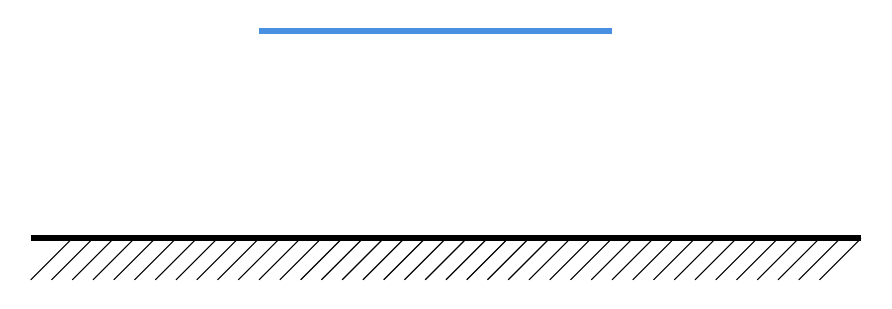
\begin{tikzpicture}[x=0.75pt,y=0.75pt,yscale=-1,xscale=1]
	%uncomment if require: \path (0,144); %set diagram left start at 0, and has height of 144
	
	%Straight Lines [id:da19142321097236792] 
	\draw [line width=2.25]    (110,110) -- (510,110) ;
	%Straight Lines [id:da6924235381108965] 
	\draw    (130,110) -- (110,130) ;
	%Straight Lines [id:da06754398351215163] 
	\draw    (140,110) -- (120,130) ;
	%Straight Lines [id:da05353958727844965] 
	\draw    (150,110) -- (130,130) ;
	%Straight Lines [id:da9799285575253245] 
	\draw    (160,110) -- (140,130) ;
	%Straight Lines [id:da1673500841222859] 
	\draw    (170,110) -- (150,130) ;
	%Straight Lines [id:da15631894580301942] 
	\draw    (180,110) -- (160,130) ;
	%Straight Lines [id:da74770424340761] 
	\draw    (190,110) -- (170,130) ;
	%Straight Lines [id:da6625553967151789] 
	\draw    (200,110) -- (180,130) ;
	%Straight Lines [id:da6964060835072168] 
	\draw    (210,110) -- (190,130) ;
	%Straight Lines [id:da2142763347370491] 
	\draw    (220,110) -- (200,130) ;
	%Straight Lines [id:da5361200634544281] 
	\draw    (230,110) -- (210,130) ;
	%Straight Lines [id:da6289898300908565] 
	\draw    (240,110) -- (220,130) ;
	%Straight Lines [id:da7639217090794013] 
	\draw    (250,110) -- (230,130) ;
	%Straight Lines [id:da43101159785028087] 
	\draw    (260,110) -- (240,130) ;
	%Straight Lines [id:da8335315550877818] 
	\draw    (270,110) -- (250,130) ;
	%Straight Lines [id:da19147462127275272] 
	\draw    (280,110) -- (260,130) ;
	%Straight Lines [id:da07753836724411789] 
	\draw    (290,110) -- (270,130) ;
	%Straight Lines [id:da49278394737292186] 
	\draw    (300,110) -- (280,130) ;
	%Straight Lines [id:da597832078560091] 
	\draw    (310,110) -- (290,130) ;
	%Straight Lines [id:da46741396957908243] 
	\draw    (320,110) -- (300,130) ;
	%Straight Lines [id:da408437076106271] 
	\draw    (330,110) -- (310,130) ;
	%Straight Lines [id:da6468877469838277] 
	\draw    (340,110) -- (320,130) ;
	%Straight Lines [id:da1515496875484319] 
	\draw    (350,110) -- (330,130) ;
	%Straight Lines [id:da7601285287056747] 
	\draw    (360,110) -- (340,130) ;
	%Straight Lines [id:da8753915548370792] 
	\draw    (370,110) -- (350,130) ;
	%Straight Lines [id:da03894040052460146] 
	\draw    (380,110) -- (360,130) ;
	%Straight Lines [id:da18654880215680536] 
	\draw    (390,110) -- (370,130) ;
	%Straight Lines [id:da394942910957522] 
	\draw    (400,110) -- (380,130) ;
	%Straight Lines [id:da1672593802412956] 
	\draw    (410,110) -- (390,130) ;
	%Straight Lines [id:da05772486377885255] 
	\draw    (420,110) -- (400,130) ;
	%Straight Lines [id:da49187521356559905] 
	\draw    (430,110) -- (410,130) ;
	%Straight Lines [id:da834562736813218] 
	\draw    (440,110) -- (420,130) ;
	%Straight Lines [id:da7470275272845139] 
	\draw    (450,110) -- (430,130) ;
	%Straight Lines [id:da8553633319133338] 
	\draw    (460,110) -- (440,130) ;
	%Straight Lines [id:da8670605086731122] 
	\draw    (470,110) -- (450,130) ;
	%Straight Lines [id:da8349863080348996] 
	\draw    (480,110) -- (460,130) ;
	%Straight Lines [id:da1809512268503919] 
	\draw    (490,110) -- (470,130) ;
	%Straight Lines [id:da5589817721122612] 
	\draw    (500,110) -- (480,130) ;
	%Straight Lines [id:da3160690002296842] 
	\draw    (510,110) -- (490,130) ;
	%Straight Lines [id:da3928674836828301] 
	\draw [color={rgb, 255:red, 74; green, 144; blue, 226 }  ,draw opacity=1 ][line width=2.25]    (220,10) -- (390,10) ;
	
\end{tikzpicture}
\caption{第一条原则}
\end{figure}


\item 只要刚性连接的都看成一根杆。
\begin{figure}[!ht]
	\centering
\tikzset{every picture/.style={line width=0.75pt}} %set default line width to 0.75pt        

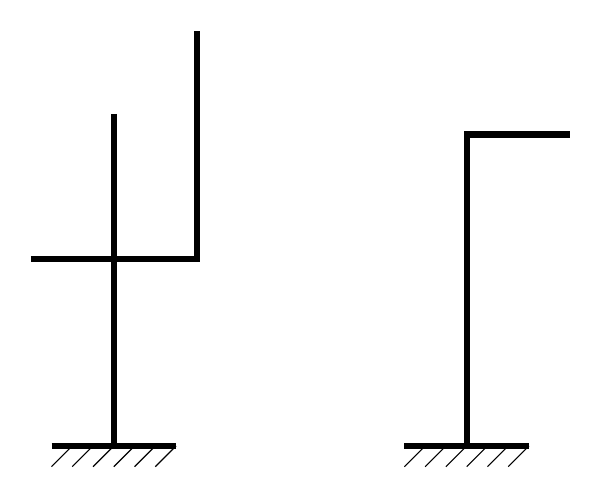
\begin{tikzpicture}[x=0.75pt,y=0.75pt,yscale=-1,xscale=1]
	%uncomment if require: \path (0,243); %set diagram left start at 0, and has height of 243
	
	%Straight Lines [id:da48723828101034194] 
	\draw [line width=2.25]    (210,210) -- (270,210) ;
	%Straight Lines [id:da9181027120373297] 
	\draw [line width=2.25]    (240,50) -- (240,210) ;
	%Straight Lines [id:da602622313919287] 
	\draw [line width=2.25]    (200,120) -- (280,120)-- (280,10) ;
	%Straight Lines [id:da9240962643084318] 
	\draw [line width=2.25]    (380,210) -- (440,210) ;
	%Straight Lines [id:da6088177156525376] 
	\draw [line width=2.25]    (410,210) -- (410,60)-- (460,60) ;
	%Straight Lines [id:da18772355497010085] 
	\draw    (230,210) -- (220,220) ;
	%Straight Lines [id:da4111734204635673] 
	\draw    (220,210) -- (210,220) ;
	%Straight Lines [id:da22170283469466634] 
	\draw    (250,210) -- (240,220) ;
	%Straight Lines [id:da37045531210319527] 
	\draw    (240,210) -- (230,220) ;
	%Straight Lines [id:da3409018442815923] 
	\draw    (270,210) -- (260,220) ;
	%Straight Lines [id:da5614281144127149] 
	\draw    (260,210) -- (250,220) ;
	%Straight Lines [id:da4814860558051475] 
	\draw    (400,210) -- (390,220) ;
	%Straight Lines [id:da24775805984689558] 
	\draw    (390,210) -- (380,220) ;
	%Straight Lines [id:da5468227638976404] 
	\draw    (420,210) -- (410,220) ;
	%Straight Lines [id:da8736964963523615] 
	\draw    (410,210) -- (400,220) ;
	%Straight Lines [id:da8905437847943618] 
	\draw    (440,210) -- (430,220) ;
	%Straight Lines [id:da39185002883344033] 
	\draw    (430,210) -- (420,220) ;
	
\end{tikzpicture}
\caption{第二条原则}
\end{figure}


\item 刚性节点看成3个约束,刚性封闭框格也看成3个约束。
\begin{figure}[!ht]
	\centering
\tikzset{every picture/.style={line width=0.75pt}} %set default line width to 0.75pt        

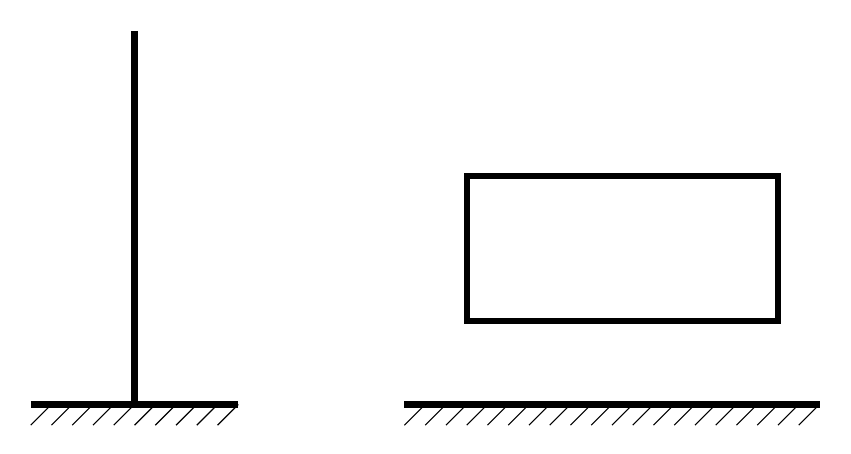
\begin{tikzpicture}[x=0.75pt,y=0.75pt,yscale=-1,xscale=1]
	%uncomment if require: \path (0,234); %set diagram left start at 0, and has height of 234
	
	%Straight Lines [id:da1494206630363457] 
	\draw [line width=2.25]    (140,200) -- (240,200) ;
	%Straight Lines [id:da021038683819858628] 
	\draw [line width=2.25]    (190,20) -- (190,200) ;
	%Straight Lines [id:da6437333320834968] 
	\draw    (140,210) -- (150,200) ;
	%Straight Lines [id:da04598717292338339] 
	\draw    (150,210) -- (160,200) ;
	%Straight Lines [id:da057725790041922576] 
	\draw    (160,210) -- (170,200) ;
	%Straight Lines [id:da12188365586198291] 
	\draw    (170,210) -- (180,200) ;
	%Straight Lines [id:da6384772771066007] 
	\draw    (180,210) -- (190,200) ;
	%Straight Lines [id:da6270858296097501] 
	\draw    (190,210) -- (200,200) ;
	%Straight Lines [id:da7291068701837558] 
	\draw    (200,210) -- (210,200) ;
	%Straight Lines [id:da9173213173554711] 
	\draw    (210,210) -- (220,200) ;
	%Straight Lines [id:da24059052404723258] 
	\draw    (220,210) -- (230,200) ;
	%Straight Lines [id:da33228461820253474] 
	\draw    (230,210) -- (240,200) ;
	%Straight Lines [id:da29709537451612844] 
	\draw [line width=2.25]    (320,200) -- (420,200) ;
	%Straight Lines [id:da01947431895506302] 
	\draw    (320,210) -- (330,200) ;
	%Straight Lines [id:da19400504371362426] 
	\draw    (330,210) -- (340,200) ;
	%Straight Lines [id:da5685365967757696] 
	\draw    (340,210) -- (350,200) ;
	%Straight Lines [id:da7406641383381025] 
	\draw    (350,210) -- (360,200) ;
	%Straight Lines [id:da8270353077372523] 
	\draw    (360,210) -- (370,200) ;
	%Straight Lines [id:da6479397769943023] 
	\draw    (370,210) -- (380,200) ;
	%Straight Lines [id:da49645436249634667] 
	\draw    (380,210) -- (390,200) ;
	%Straight Lines [id:da3702297825653882] 
	\draw    (390,210) -- (400,200) ;
	%Straight Lines [id:da17210221936369385] 
	\draw    (400,210) -- (410,200) ;
	%Straight Lines [id:da5254368727523482] 
	\draw    (410,210) -- (420,200) ;
	%Straight Lines [id:da6489335975911368] 
	\draw [line width=2.25]    (420,200) -- (520,200) ;
	%Straight Lines [id:da6011696339904511] 
	\draw    (420,210) -- (430,200) ;
	%Straight Lines [id:da3438004738519771] 
	\draw    (430,210) -- (440,200) ;
	%Straight Lines [id:da09185455292510825] 
	\draw    (440,210) -- (450,200) ;
	%Straight Lines [id:da436741128707431] 
	\draw    (450,210) -- (460,200) ;
	%Straight Lines [id:da17578128972263207] 
	\draw    (460,210) -- (470,200) ;
	%Straight Lines [id:da543290232241731] 
	\draw    (470,210) -- (480,200) ;
	%Straight Lines [id:da16264624135224204] 
	\draw    (480,210) -- (490,200) ;
	%Straight Lines [id:da5032217662761382] 
	\draw    (490,210) -- (500,200) ;
	%Straight Lines [id:da19134027955433153] 
	\draw    (500,210) -- (510,200) ;
	%Straight Lines [id:da5675548470527982] 
	\draw    (510,210) -- (520,200) ;
	%Shape: Rectangle [id:dp022641157747854024] 
	\draw  [line width=2.25]  (350,90) -- (500,90) -- (500,160) -- (350,160) -- cycle ;
	
	
\end{tikzpicture}
\caption{第三条原则}
\end{figure}


\item 一个铰接点看成两个约束。
\begin{figure}[!ht]
	\centering
\tikzset{every picture/.style={line width=0.75pt}} %set default line width to 0.75pt        

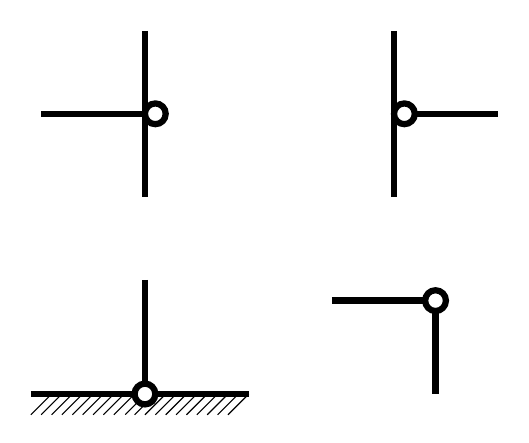
\begin{tikzpicture}[x=0.75pt,y=0.75pt,yscale=-1,xscale=1]
	%uncomment if require: \path (0,225); %set diagram left start at 0, and has height of 225
	
	%Straight Lines [id:da7495306508589998] 
	\draw [line width=2.25]    (250,15) -- (250,95) ;
	%Straight Lines [id:da0004590644200239691] 
	\draw [line width=2.25]    (200,55) -- (250,55) ;
	%Shape: Circle [id:dp27954834617974855] 
	\draw  [line width=2.25]  (250,55) .. controls (250,52.24) and (252.24,50) .. (255,50) .. controls (257.76,50) and (260,52.24) .. (260,55) .. controls (260,57.76) and (257.76,60) .. (255,60) .. controls (252.24,60) and (250,57.76) .. (250,55) -- cycle ;
	%Straight Lines [id:da43820486304875406] 
	\draw [line width=2.25]    (370,15) -- (370,95) ;
	%Shape: Circle [id:dp1653818479346405] 
	\draw  [line width=2.25]  (370,55) .. controls (370,52.24) and (372.24,50) .. (375,50) .. controls (377.76,50) and (380,52.24) .. (380,55) .. controls (380,57.76) and (377.76,60) .. (375,60) .. controls (372.24,60) and (370,57.76) .. (370,55) -- cycle ;
	%Straight Lines [id:da9474388544997172] 
	\draw [line width=2.25]    (380,55) -- (420,55) ;
	%Straight Lines [id:da8207995915439157] 
	\draw [line width=2.25]    (255,190) -- (300,190) ;
	%Straight Lines [id:da24832170430256295] 
	\draw [line width=2.25]    (250,135) -- (250,185) ;
	%Shape: Circle [id:dp950836324956635] 
	\draw  [line width=2.25]  (245,190) .. controls (245,187.24) and (247.24,185) .. (250,185) .. controls (252.76,185) and (255,187.24) .. (255,190) .. controls (255,192.76) and (252.76,195) .. (250,195) .. controls (247.24,195) and (245,192.76) .. (245,190) -- cycle ;
	%Straight Lines [id:da20767079793157217] 
	\draw [line width=2.25]    (195,190) -- (245,190) ;
	%Straight Lines [id:da67856168253064] 
	\draw    (205,190) -- (195,200) ;
	%Straight Lines [id:da8269844492241123] 
	\draw    (210,190) -- (200,200) ;
	%Straight Lines [id:da5520780633357969] 
	\draw    (215,190) -- (205,200) ;
	%Straight Lines [id:da3110548979040937] 
	\draw    (220,190) -- (210,200) ;
	%Straight Lines [id:da2437318948912921] 
	\draw    (225,190) -- (215,200) ;
	%Straight Lines [id:da16138152432547614] 
	\draw    (230,190) -- (220,200) ;
	%Straight Lines [id:da9976779088439263] 
	\draw    (235,190) -- (225,200) ;
	%Straight Lines [id:da2860931698295972] 
	\draw    (240,190) -- (230,200) ;
	%Straight Lines [id:da09703262828007042] 
	\draw    (245,190) -- (235,200) ;
	%Straight Lines [id:da9506295823364495] 
	\draw    (260,190) -- (250,200) ;
	%Straight Lines [id:da8289995329213529] 
	\draw    (265,190) -- (255,200) ;
	%Straight Lines [id:da9315047008315245] 
	\draw    (270,190) -- (260,200) ;
	%Straight Lines [id:da8689083923793353] 
	\draw    (275,190) -- (265,200) ;
	%Straight Lines [id:da9894480469151854] 
	\draw    (280,190) -- (270,200) ;
	%Straight Lines [id:da6030150323123316] 
	\draw    (285,190) -- (275,200) ;
	%Straight Lines [id:da5270374873518371] 
	\draw    (290,190) -- (280,200) ;
	%Straight Lines [id:da9828122738641056] 
	\draw    (295,190) -- (285,200) ;
	%Straight Lines [id:da9117856715321269] 
	\draw    (300,190) -- (290,200) ;
	%Straight Lines [id:da8886518239950592] 
	\draw [line width=2.25]    (340,145) -- (385,145) ;
	%Shape: Circle [id:dp7986495199828691] 
	\draw  [line width=2.25]  (385,145) .. controls (385,142.24) and (387.24,140) .. (390,140) .. controls (392.76,140) and (395,142.24) .. (395,145) .. controls (395,147.76) and (392.76,150) .. (390,150) .. controls (387.24,150) and (385,147.76) .. (385,145) -- cycle ;
	%Straight Lines [id:da3436002039309032] 
	\draw [line width=2.25]    (390,150) -- (390,190) ;
	%Straight Lines [id:da4255271061782404] 
	\draw    (250,195) -- (245,200) ;
	%Straight Lines [id:da09365524036838879] 
	\draw    (247.01,193.41) -- (240.51,199.91) ;
	
\end{tikzpicture}
\caption{第四条原则}
\end{figure}


\item $\displaystyle N$个连杆铰接,算$\displaystyle N-1$个铰接点。
\item 组合式铰链可以分解计算。
\begin{figure}[!ht]
	\centering
\tikzset{every picture/.style={line width=0.75pt}} %set default line width to 0.75pt        

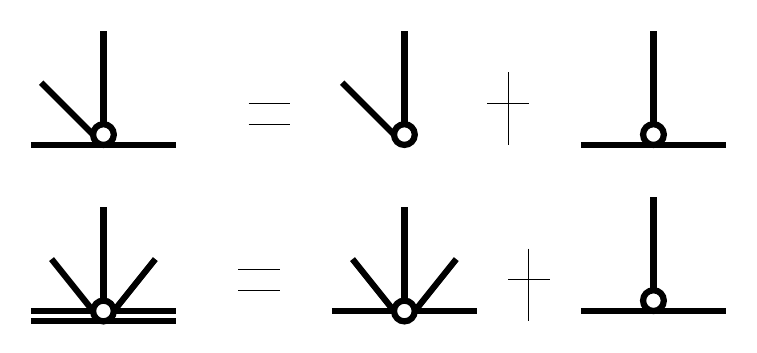
\begin{tikzpicture}[x=0.75pt,y=0.75pt,yscale=-1,xscale=1]
	%uncomment if require: \path (0,188); %set diagram left start at 0, and has height of 188
	
	%Straight Lines [id:da22317063315639074] 
	\draw [line width=2.25]    (160,75) -- (230,75) ;
	%Shape: Circle [id:dp9489222136216069] 
	\draw  [line width=2.25]  (190,70) .. controls (190,67.24) and (192.24,65) .. (195,65) .. controls (197.76,65) and (200,67.24) .. (200,70) .. controls (200,72.76) and (197.76,75) .. (195,75) .. controls (192.24,75) and (190,72.76) .. (190,70) -- cycle ;
	%Straight Lines [id:da20583145498241162] 
	\draw [line width=2.25]    (195,65) -- (195,20) ;
	%Straight Lines [id:da49673336594197814] 
	\draw [line width=2.25]    (165,45) -- (190,70) ;
	%Straight Lines [id:da285413877471715] 
	\draw    (265,55) -- (285,55) ;
	%Straight Lines [id:da8188364451016874] 
	\draw    (265,65) -- (285,65) ;
	%Shape: Circle [id:dp653456399289231] 
	\draw  [line width=2.25]  (335,70) .. controls (335,67.24) and (337.24,65) .. (340,65) .. controls (342.76,65) and (345,67.24) .. (345,70) .. controls (345,72.76) and (342.76,75) .. (340,75) .. controls (337.24,75) and (335,72.76) .. (335,70) -- cycle ;
	%Straight Lines [id:da9728875511808333] 
	\draw [line width=2.25]    (340,65) -- (340,20) ;
	%Straight Lines [id:da5379619411836745] 
	\draw [line width=2.25]    (310,45) -- (335,70) ;
	%Straight Lines [id:da990059257334768] 
	\draw    (380,55) -- (400,55) ;
	%Straight Lines [id:da5129400373430522] 
	\draw    (390,40) -- (390,75) ;
	%Straight Lines [id:da9355451773133447] 
	\draw [line width=2.25]    (425,75) -- (495,75) ;
	%Shape: Circle [id:dp11432021175312213] 
	\draw  [line width=2.25]  (455,70) .. controls (455,67.24) and (457.24,65) .. (460,65) .. controls (462.76,65) and (465,67.24) .. (465,70) .. controls (465,72.76) and (462.76,75) .. (460,75) .. controls (457.24,75) and (455,72.76) .. (455,70) -- cycle ;
	%Straight Lines [id:da8859230358800001] 
	\draw [line width=2.25]    (460,65) -- (460,20) ;
	%Straight Lines [id:da31215157818751194] 
	\draw [line width=2.25]    (160,160) -- (230,160) ;
	%Shape: Circle [id:dp5808272231115363] 
	\draw  [line width=2.25]  (190,155) .. controls (190,152.24) and (192.24,150) .. (195,150) .. controls (197.76,150) and (200,152.24) .. (200,155) .. controls (200,157.76) and (197.76,160) .. (195,160) .. controls (192.24,160) and (190,157.76) .. (190,155) -- cycle ;
	%Straight Lines [id:da6298355434059231] 
	\draw [line width=2.25]    (195,150) -- (195,105) ;
	%Straight Lines [id:da8001944987706804] 
	\draw [line width=2.25]    (170,130) -- (190,155) ;
	%Straight Lines [id:da5246616482260829] 
	\draw [line width=2.25]    (160,155) -- (190,155) ;
	%Straight Lines [id:da2919646235467013] 
	\draw [line width=2.25]    (200,155) -- (230,155) ;
	%Straight Lines [id:da2400442486059513] 
	\draw [line width=2.25]    (200,155) -- (220,130) ;
	%Straight Lines [id:da6721942655766391] 
	\draw    (260,135) -- (280,135) ;
	%Straight Lines [id:da4448569884443778] 
	\draw    (260,145) -- (280,145) ;
	%Shape: Circle [id:dp36494815010853787] 
	\draw  [line width=2.25]  (335,155) .. controls (335,152.24) and (337.24,150) .. (340,150) .. controls (342.76,150) and (345,152.24) .. (345,155) .. controls (345,157.76) and (342.76,160) .. (340,160) .. controls (337.24,160) and (335,157.76) .. (335,155) -- cycle ;
	%Straight Lines [id:da5657859649112764] 
	\draw [line width=2.25]    (340,150) -- (340,105) ;
	%Straight Lines [id:da5555589513444292] 
	\draw [line width=2.25]    (315,130) -- (335,155) ;
	%Straight Lines [id:da06438649379908123] 
	\draw [line width=2.25]    (305,155) -- (335,155) ;
	%Straight Lines [id:da6627977154856652] 
	\draw [line width=2.25]    (345,155) -- (375,155) ;
	%Straight Lines [id:da9999680845849797] 
	\draw [line width=2.25]    (345,155) -- (365,130) ;
	%Straight Lines [id:da8827320005031338] 
	\draw [line width=2.25]    (425,155) -- (495,155) ;
	%Shape: Circle [id:dp7062653938850874] 
	\draw  [line width=2.25]  (455,150) .. controls (455,147.24) and (457.24,145) .. (460,145) .. controls (462.76,145) and (465,147.24) .. (465,150) .. controls (465,152.76) and (462.76,155) .. (460,155) .. controls (457.24,155) and (455,152.76) .. (455,150) -- cycle ;
	%Straight Lines [id:da3725659895410498] 
	\draw [line width=2.25]    (460,145) -- (460,100) ;
	%Straight Lines [id:da41287463765411303] 
	\draw    (390,140) -- (410,140) ;
	%Straight Lines [id:da6770309244838046] 
	\draw    (400,125) -- (400,160) ;
	
\end{tikzpicture}
\caption{第六条原则}
\end{figure}
 \end{enumerate}

\section{计算规则}
\begin{enumerate}
\item 分析有几个独立杆件,按照原则2判定;

\item 计算独立的杆件有几根,乘3就是静定所需的约束数;

\item 计算杆件和地面的独立刚节点,乘3就是约束数;计算独立杆件和地面的铰接点,乘2就是约束数;如果有刚性封闭框格,乘3就是约束数;

\item 约束数减去静定约束数量就是超静定次数;
\end{enumerate}
\section{计算讲解}
\begin{enumerate}
	\item 
	\begin{figure}[!ht]
		\centering
\tikzset{every picture/.style={line width=0.75pt}} %set default line width to 0.75pt        

\begin{tikzpicture}[x=0.75pt,y=0.75pt,yscale=-1,xscale=1]
	%uncomment if require: \path (0,150); %set diagram left start at 0, and has height of 150
	
	%Shape: Circle [id:dp9914182276372867] 
	\draw  [line width=2.25]  (185,40) .. controls (185,37.24) and (187.24,35) .. (190,35) .. controls (192.76,35) and (195,37.24) .. (195,40) .. controls (195,42.76) and (192.76,45) .. (190,45) .. controls (187.24,45) and (185,42.76) .. (185,40) -- cycle ;
	%Shape: Circle [id:dp8016647757210809] 
	\draw  [line width=2.25]  (215,40) .. controls (215,37.24) and (217.24,35) .. (220,35) .. controls (222.76,35) and (225,37.24) .. (225,40) .. controls (225,42.76) and (222.76,45) .. (220,45) .. controls (217.24,45) and (215,42.76) .. (215,40) -- cycle ;
	%Straight Lines [id:da18362914864003743] 
	\draw [line width=2.25]    (170,40) -- (185,40) ;
	%Straight Lines [id:da4933046172461768] 
	\draw [line width=2.25]    (195,40) -- (215,40) ;
	%Straight Lines [id:da2711141890639779] 
	\draw [line width=2.25]    (225,40) -- (240,40) ;
	%Straight Lines [id:da32562115568615746] 
	\draw [line width=2.25]    (202.11,19.09) -- (192.51,35.49) ;
	%Shape: Circle [id:dp10414866216305319] 
	\draw  [line width=2.25]  (200,15) .. controls (200,12.24) and (202.24,10) .. (205,10) .. controls (207.76,10) and (210,12.24) .. (210,15) .. controls (210,17.76) and (207.76,20) .. (205,20) .. controls (202.24,20) and (200,17.76) .. (200,15) -- cycle ;
	%Straight Lines [id:da5873683565737926] 
	\draw [line width=2.25]    (207.31,18.69) -- (216.91,35.49) ;
	%Straight Lines [id:da6122438296070845] 
	\draw [line width=2.25]    (210,15) -- (340,15) ;
	%Shape: Circle [id:dp998731562932277] 
	\draw  [line width=2.25]  (340,15) .. controls (340,12.24) and (342.24,10) .. (345,10) .. controls (347.76,10) and (350,12.24) .. (350,15) .. controls (350,17.76) and (347.76,20) .. (345,20) .. controls (342.24,20) and (340,17.76) .. (340,15) -- cycle ;
	%Straight Lines [id:da285750534125607] 
	\draw [line width=2.25]    (345,20) -- (345,35) ;
	%Shape: Circle [id:dp8643094970594003] 
	\draw  [line width=2.25]  (340,40) .. controls (340,37.24) and (342.24,35) .. (345,35) .. controls (347.76,35) and (350,37.24) .. (350,40) .. controls (350,42.76) and (347.76,45) .. (345,45) .. controls (342.24,45) and (340,42.76) .. (340,40) -- cycle ;
	%Straight Lines [id:da013884097629328185] 
	\draw [line width=2.25]    (350,40) -- (370,40) ;
	%Straight Lines [id:da4379233825227673] 
	\draw [line width=2.25]    (320,40) -- (340,40) ;
	%Straight Lines [id:da050331560047672586] 
	\draw    (175,40) -- (170,45) ;
	%Straight Lines [id:da5517772901304674] 
	\draw    (180,40) -- (175,45) ;
	%Straight Lines [id:da316868350624264] 
	\draw    (185,40) -- (180,45) ;
	%Straight Lines [id:da0055372853104704856] 
	\draw    (200,40) -- (195,45) ;
	%Straight Lines [id:da9878254867743188] 
	\draw    (205,40) -- (200,45) ;
	%Straight Lines [id:da9680340560547118] 
	\draw    (210,40) -- (205,45) ;
	%Straight Lines [id:da34070066708396585] 
	\draw    (215,40) -- (210,45) ;
	%Straight Lines [id:da6403315980082345] 
	\draw    (230,40) -- (225,45) ;
	%Straight Lines [id:da321219972932689] 
	\draw    (235,40) -- (230,45) ;
	%Straight Lines [id:da7995635215222967] 
	\draw    (240,40) -- (235,45) ;
	%Straight Lines [id:da9215992744839685] 
	\draw    (325,40) -- (320,45) ;
	%Straight Lines [id:da2812531761231982] 
	\draw    (330,40) -- (325,45) ;
	%Straight Lines [id:da4032182147598755] 
	\draw    (335,40) -- (330,45) ;
	%Straight Lines [id:da6243992642409588] 
	\draw    (340,40) -- (335,45) ;
	%Straight Lines [id:da6384236910934022] 
	\draw    (355,40) -- (350,45) ;
	%Straight Lines [id:da5327993153676476] 
	\draw    (360,40) -- (355,45) ;
	%Straight Lines [id:da8493258949179276] 
	\draw    (365,40) -- (360,45) ;
	%Straight Lines [id:da07197380753727045] 
	\draw    (370,40) -- (365,45) ;
	%Shape: Circle [id:dp6897680758787883] 
	\draw  [line width=2.25]  (185,105) .. controls (185,102.24) and (187.24,100) .. (190,100) .. controls (192.76,100) and (195,102.24) .. (195,105) .. controls (195,107.76) and (192.76,110) .. (190,110) .. controls (187.24,110) and (185,107.76) .. (185,105) -- cycle ;
	%Shape: Circle [id:dp42195267814734905] 
	\draw  [line width=2.25]  (215,105) .. controls (215,102.24) and (217.24,100) .. (220,100) .. controls (222.76,100) and (225,102.24) .. (225,105) .. controls (225,107.76) and (222.76,110) .. (220,110) .. controls (217.24,110) and (215,107.76) .. (215,105) -- cycle ;
	%Straight Lines [id:da6902342346200661] 
	\draw [line width=2.25]    (170,105) -- (185,105) ;
	%Straight Lines [id:da9657095873534995] 
	\draw [line width=2.25]    (195,105) -- (215,105) ;
	%Straight Lines [id:da2165486146188269] 
	\draw [line width=2.25]    (225,105) -- (240,105) ;
	%Straight Lines [id:da10339878228696708] 
	\draw [line width=2.25]    (202.11,84.09) -- (192.51,100.49) ;
	%Shape: Circle [id:dp9909002560822875] 
	\draw  [line width=2.25]  (200,80) .. controls (200,77.24) and (202.24,75) .. (205,75) .. controls (207.76,75) and (210,77.24) .. (210,80) .. controls (210,82.76) and (207.76,85) .. (205,85) .. controls (202.24,85) and (200,82.76) .. (200,80) -- cycle ;
	%Straight Lines [id:da8879342100630068] 
	\draw [line width=2.25]    (207.31,83.69) -- (216.91,100.49) ;
	%Straight Lines [id:da3927764270501517] 
	\draw [line width=2.25]    (210,80) -- (340,80) ;
	%Shape: Circle [id:dp6732081377782273] 
	\draw  [line width=2.25]  (340,80) .. controls (340,77.24) and (342.24,75) .. (345,75) .. controls (347.76,75) and (350,77.24) .. (350,80) .. controls (350,82.76) and (347.76,85) .. (345,85) .. controls (342.24,85) and (340,82.76) .. (340,80) -- cycle ;
	%Straight Lines [id:da3628372644182305] 
	\draw [line width=2.25]    (345,85) -- (345,100) ;
	%Shape: Circle [id:dp01818429868303073] 
	\draw  [line width=2.25]  (340,105) .. controls (340,102.24) and (342.24,100) .. (345,100) .. controls (347.76,100) and (350,102.24) .. (350,105) .. controls (350,107.76) and (347.76,110) .. (345,110) .. controls (342.24,110) and (340,107.76) .. (340,105) -- cycle ;
	%Straight Lines [id:da26581419831396746] 
	\draw [line width=2.25]    (350,105) -- (370,105) ;
	%Straight Lines [id:da37792553011290275] 
	\draw [line width=2.25]    (320,105) -- (340,105) ;
	%Straight Lines [id:da21034468031376785] 
	\draw    (175,105) -- (170,110) ;
	%Straight Lines [id:da1437802844020426] 
	\draw    (180,105) -- (175,110) ;
	%Straight Lines [id:da7661815682433819] 
	\draw    (185,105) -- (180,110) ;
	%Straight Lines [id:da736235423281284] 
	\draw    (200,105) -- (195,110) ;
	%Straight Lines [id:da2708379314427376] 
	\draw    (205,105) -- (200,110) ;
	%Straight Lines [id:da11525260129749548] 
	\draw    (210,105) -- (205,110) ;
	%Straight Lines [id:da09009400744407436] 
	\draw    (215,105) -- (210,110) ;
	%Straight Lines [id:da49628465884200734] 
	\draw    (230,105) -- (225,110) ;
	%Straight Lines [id:da061512995343041554] 
	\draw    (235,105) -- (230,110) ;
	%Straight Lines [id:da6359910752574212] 
	\draw    (240,105) -- (235,110) ;
	%Straight Lines [id:da5273528296671772] 
	\draw    (325,105) -- (320,110) ;
	%Straight Lines [id:da21285129509789935] 
	\draw    (330,105) -- (325,110) ;
	%Straight Lines [id:da3339925878629304] 
	\draw    (335,105) -- (330,110) ;
	%Straight Lines [id:da3261037098825197] 
	\draw    (340,105) -- (335,110) ;
	%Straight Lines [id:da38906066370412895] 
	\draw    (355,105) -- (350,110) ;
	%Straight Lines [id:da50648220688569] 
	\draw    (360,105) -- (355,110) ;
	%Straight Lines [id:da4506439647752649] 
	\draw    (365,105) -- (360,110) ;
	%Straight Lines [id:da8329875654515277] 
	\draw    (370,105) -- (365,110) ;
	
	% Text Node
	\draw (175,87) node [anchor=north west][inner sep=0.75pt]  [font=\fontsize{0.53em}{0.64em}\selectfont] [align=left] {杆1};
	% Text Node
	\draw (216,87) node [anchor=north west][inner sep=0.75pt]  [font=\fontsize{0.53em}{0.64em}\selectfont] [align=left] {杆1};
	% Text Node
	\draw (266,68) node [anchor=north west][inner sep=0.75pt]  [font=\fontsize{0.53em}{0.64em}\selectfont] [align=left] {杆1};
	% Text Node
	\draw (347,88) node [anchor=north west][inner sep=0.75pt]  [font=\fontsize{0.53em}{0.64em}\selectfont] [align=left] {杆1};
	% Text Node
	\draw (201,63) node [anchor=north west][inner sep=0.75pt]  [font=\fontsize{0.53em}{0.64em}\selectfont] [align=left] {铰2};
	% Text Node
	\draw (182,113) node [anchor=north west][inner sep=0.75pt]  [font=\fontsize{0.53em}{0.64em}\selectfont] [align=left] {铰1};
	% Text Node
	\draw (212,113) node [anchor=north west][inner sep=0.75pt]  [font=\fontsize{0.53em}{0.64em}\selectfont] [align=left] {铰1};
	% Text Node
	\draw (336,63) node [anchor=north west][inner sep=0.75pt]  [font=\fontsize{0.53em}{0.64em}\selectfont] [align=left] {铰1};
	% Text Node
	\draw (337,113) node [anchor=north west][inner sep=0.75pt]  [font=\fontsize{0.53em}{0.64em}\selectfont] [align=left] {铰1};
	
\end{tikzpicture}
\caption{题图1}
\end{figure}
4根杆件,需要$\displaystyle 3\times 4=12$个约束;6个铰,共$\displaystyle 6\times 2=12$个约束,静定。

\item 
\begin{figure}[!ht]
	\centering
\tikzset{every picture/.style={line width=0.75pt}} %set default line width to 0.75pt        

\begin{tikzpicture}[x=0.75pt,y=0.75pt,yscale=-1,xscale=1]
	%uncomment if require: \path (0,300); %set diagram left start at 0, and has height of 300
	
	%Straight Lines [id:da7637584054348636] 
	\draw [line width=2.25]    (114,155) -- (114,170) ;
	%Shape: Circle [id:dp7403286552960038] 
	\draw  [line width=2.25]  (109,175) .. controls (109,172.24) and (111.24,170) .. (114,170) .. controls (116.76,170) and (119,172.24) .. (119,175) .. controls (119,177.76) and (116.76,180) .. (114,180) .. controls (111.24,180) and (109,177.76) .. (109,175) -- cycle ;
	%Straight Lines [id:da5534934091686219] 
	\draw [line width=2.25]    (114,180) -- (114,195) ;
	%Straight Lines [id:da8562095168105262] 
	\draw [line width=2.25]    (119,175) -- (134,175) ;
	%Shape: Circle [id:dp3019921419913527] 
	\draw  [line width=2.25]  (134,175) .. controls (134,172.24) and (136.24,170) .. (139,170) .. controls (141.76,170) and (144,172.24) .. (144,175) .. controls (144,177.76) and (141.76,180) .. (139,180) .. controls (136.24,180) and (134,177.76) .. (134,175) -- cycle ;
	%Straight Lines [id:da7424238245600134] 
	\draw [line width=2.25]    (139,180) -- (139,195) ;
	%Shape: Circle [id:dp6493364599828684] 
	\draw  [line width=2.25]  (134,200) .. controls (134,197.24) and (136.24,195) .. (139,195) .. controls (141.76,195) and (144,197.24) .. (144,200) .. controls (144,202.76) and (141.76,205) .. (139,205) .. controls (136.24,205) and (134,202.76) .. (134,200) -- cycle ;
	%Straight Lines [id:da04749018352898071] 
	\draw [line width=2.25]    (134,200) -- (119,200) ;
	%Straight Lines [id:da079002228020574] 
	\draw [line width=2.25]    (144,200) -- (159,200) ;
	%Straight Lines [id:da7461781062527937] 
	\draw [line width=2.25]    (139,170) -- (139,100)--(164,80) ;
	%Shape: Circle [id:dp07267328808005824] 
	\draw  [line width=2.25]  (164,80) .. controls (164,77.24) and (166.24,75) .. (169,75) .. controls (171.76,75) and (174,77.24) .. (174,80) .. controls (174,82.76) and (171.76,85) .. (169,85) .. controls (166.24,85) and (164,82.76) .. (164,80) -- cycle ;
	%Straight Lines [id:da009934043155127359] 
	\draw [line width=2.25]    (164,175) -- (184,175) ;
	%Straight Lines [id:da61956142167679] 
	\draw [line width=2.25]    (189.68,49.41)--(174,60) -- (174,175) ;
	%Shape: Circle [id:dp4597205490392009] 
	\draw  [line width=2.25]  (189.5,48) .. controls (189.5,45.24) and (191.74,43) .. (194.5,43) .. controls (197.26,43) and (199.5,45.24) .. (199.5,48) .. controls (199.5,50.76) and (197.26,53) .. (194.5,53) .. controls (191.74,53) and (189.5,50.76) .. (189.5,48) -- cycle ;
	%Straight Lines [id:da1070988873213643] 
	\draw [line width=2.25]    (198.68,45.08) -- (219,30) ;
	%Shape: Circle [id:dp8488215887475352] 
	\draw  [line width=2.25]  (218,27.67) .. controls (218,24.91) and (220.24,22.67) .. (223,22.67) .. controls (225.76,22.67) and (228,24.91) .. (228,27.67) .. controls (228,30.43) and (225.76,32.67) .. (223,32.67) .. controls (220.24,32.67) and (218,30.43) .. (218,27.67) -- cycle ;
	%Straight Lines [id:da48607158786038873] 
	\draw [line width=2.25]    (227,24) -- (254,5)-- (254,175) ;
	%Straight Lines [id:da6423924781209616] 
	\draw [line width=2.25]    (239,175) -- (269,175) ;
	%Straight Lines [id:da08639987813390859] 
	\draw    (109,160) -- (114,155) ;
	%Straight Lines [id:da45610594225215273] 
	\draw    (109,165) -- (114,160) ;
	%Straight Lines [id:da08803307470646748] 
	\draw    (109,170) -- (114,165) ;
	%Straight Lines [id:da5120222574356765] 
	\draw    (109,185) -- (114,180) ;
	%Straight Lines [id:da32590875409421227] 
	\draw    (109,190) -- (114,185) ;
	%Straight Lines [id:da8866333093245795] 
	\draw    (109,195) -- (114,190) ;
	%Straight Lines [id:da2980534124119898] 
	\draw    (119,205) -- (124,200) ;
	%Straight Lines [id:da19034693528208213] 
	\draw    (124,205) -- (129,200) ;
	%Straight Lines [id:da8321953875333166] 
	\draw    (129,205) -- (134,200) ;
	%Straight Lines [id:da8458660783523986] 
	\draw    (144,205) -- (149,200) ;
	%Straight Lines [id:da6127450746298369] 
	\draw    (149,205) -- (154,200) ;
	%Straight Lines [id:da4076568055341101] 
	\draw    (154,205) -- (159,200) ;
	%Straight Lines [id:da7888445806501094] 
	\draw    (164,180) -- (169,175) ;
	%Straight Lines [id:da30866939107003155] 
	\draw    (169,180) -- (174,175) ;
	%Straight Lines [id:da6933505928000521] 
	\draw    (174,180) -- (179,175) ;
	%Straight Lines [id:da4334051416688147] 
	\draw    (179,180) -- (184,175) ;
	%Straight Lines [id:da18248568787536756] 
	\draw    (239,180) -- (244,175) ;
	%Straight Lines [id:da2771412338867738] 
	\draw    (244,180) -- (249,175) ;
	%Straight Lines [id:da8778566418265144] 
	\draw    (249,180) -- (254,175) ;
	%Straight Lines [id:da4738801319278658] 
	\draw    (254,180) -- (259,175) ;
	%Straight Lines [id:da9454711411394303] 
	\draw    (259,180) -- (264,175) ;
	%Straight Lines [id:da5450482155303857] 
	\draw    (264,180) -- (269,175) ;
	%Straight Lines [id:da054873388327274064] 
	\draw [line width=2.25]    (364,155) -- (364,170) ;
	%Shape: Circle [id:dp24716371333640286] 
	\draw  [line width=2.25]  (359,175) .. controls (359,172.24) and (361.24,170) .. (364,170) .. controls (366.76,170) and (369,172.24) .. (369,175) .. controls (369,177.76) and (366.76,180) .. (364,180) .. controls (361.24,180) and (359,177.76) .. (359,175) -- cycle ;
	%Straight Lines [id:da43651764046393016] 
	\draw [line width=2.25]    (364,180) -- (364,195) ;
	%Straight Lines [id:da2376794126487809] 
	\draw [line width=2.25]    (369,175) -- (384,175) ;
	%Shape: Circle [id:dp12850278034368912] 
	\draw  [line width=2.25]  (384,175) .. controls (384,172.24) and (386.24,170) .. (389,170) .. controls (391.76,170) and (394,172.24) .. (394,175) .. controls (394,177.76) and (391.76,180) .. (389,180) .. controls (386.24,180) and (384,177.76) .. (384,175) -- cycle ;
	%Straight Lines [id:da7776740617858564] 
	\draw [line width=2.25]    (389,180) -- (389,195) ;
	%Shape: Circle [id:dp7177595274102815] 
	\draw  [line width=2.25]  (384,200) .. controls (384,197.24) and (386.24,195) .. (389,195) .. controls (391.76,195) and (394,197.24) .. (394,200) .. controls (394,202.76) and (391.76,205) .. (389,205) .. controls (386.24,205) and (384,202.76) .. (384,200) -- cycle ;
	%Straight Lines [id:da6987814615892838] 
	\draw [line width=2.25]    (384,200) -- (369,200) ;
	%Straight Lines [id:da08474458052218026] 
	\draw [line width=2.25]    (394,200) -- (409,200) ;
	%Straight Lines [id:da12026044428732141] 
	\draw [color={rgb, 255:red, 208; green, 2; blue, 27 }  ,draw opacity=1 ][line width=2.25]    (389,170) -- (389,100)-- (414,80) ;
	%Shape: Circle [id:dp8560318738218973] 
	\draw  [line width=2.25]  (414,80) .. controls (414,77.24) and (416.24,75) .. (419,75) .. controls (421.76,75) and (424,77.24) .. (424,80) .. controls (424,82.76) and (421.76,85) .. (419,85) .. controls (416.24,85) and (414,82.76) .. (414,80) -- cycle ;
	%Straight Lines [id:da8514782283464049] 
	\draw [line width=2.25]    (414,175) -- (434,175) ;
	%Straight Lines [id:da9312876373119325] 
	\draw [color={rgb, 255:red, 245; green, 166; blue, 35 }  ,draw opacity=1 ][line width=2.25]    (439.67,49.33)--(424,60) -- (424,175) ;
	%Shape: Circle [id:dp12837891653420574] 
	\draw  [line width=2.25]  (439.5,48) .. controls (439.5,45.24) and (441.74,43) .. (444.5,43) .. controls (447.26,43) and (449.5,45.24) .. (449.5,48) .. controls (449.5,50.76) and (447.26,53) .. (444.5,53) .. controls (441.74,53) and (439.5,50.76) .. (439.5,48) -- cycle ;
	%Straight Lines [id:da6063270705374815] 
	\draw [line width=2.25]    (448.68,45.08) -- (469,30) ;
	%Shape: Circle [id:dp6887941414929426] 
	\draw  [line width=2.25]  (468,27.67) .. controls (468,24.91) and (470.24,22.67) .. (473,22.67) .. controls (475.76,22.67) and (478,24.91) .. (478,27.67) .. controls (478,30.43) and (475.76,32.67) .. (473,32.67) .. controls (470.24,32.67) and (468,30.43) .. (468,27.67) -- cycle ;
	%Straight Lines [id:da9292587966472341] 
	\draw [color={rgb, 255:red, 74; green, 144; blue, 226 }  ,draw opacity=1 ][line width=2.25]    (477,24) -- (504,5)-- (504,175) ;
	%Straight Lines [id:da28067516290507477] 
	\draw [line width=2.25]    (489,175) -- (519,175) ;
	%Straight Lines [id:da891778097992113] 
	\draw    (359,160) -- (364,155) ;
	%Straight Lines [id:da7063785899748167] 
	\draw    (359,165) -- (364,160) ;
	%Straight Lines [id:da25053466145898295] 
	\draw    (359,170) -- (364,165) ;
	%Straight Lines [id:da7995502019059022] 
	\draw    (359,185) -- (364,180) ;
	%Straight Lines [id:da9831226426794244] 
	\draw    (359,190) -- (364,185) ;
	%Straight Lines [id:da18415416411539143] 
	\draw    (359,195) -- (364,190) ;
	%Straight Lines [id:da9761220428228994] 
	\draw    (369,205) -- (374,200) ;
	%Straight Lines [id:da40051814183181245] 
	\draw    (374,205) -- (379,200) ;
	%Straight Lines [id:da8831891405636185] 
	\draw    (379,205) -- (384,200) ;
	%Straight Lines [id:da8411012085905389] 
	\draw    (394,205) -- (399,200) ;
	%Straight Lines [id:da200790702061715] 
	\draw    (399,205) -- (404,200) ;
	%Straight Lines [id:da6129628031322918] 
	\draw    (404,205) -- (409,200) ;
	%Straight Lines [id:da7353173586046777] 
	\draw    (414,180) -- (419,175) ;
	%Straight Lines [id:da9904540615836375] 
	\draw    (419,180) -- (424,175) ;
	%Straight Lines [id:da7318069911056322] 
	\draw    (424,180) -- (429,175) ;
	%Straight Lines [id:da32391179548374627] 
	\draw    (429,180) -- (434,175) ;
	%Straight Lines [id:da4608611596174381] 
	\draw    (489,180) -- (494,175) ;
	%Straight Lines [id:da6923979028687459] 
	\draw    (494,180) -- (499,175) ;
	%Straight Lines [id:da3047112872517306] 
	\draw    (499,180) -- (504,175) ;
	%Straight Lines [id:da9918481123910363] 
	\draw    (504,180) -- (509,175) ;
	%Straight Lines [id:da9179836925630867] 
	\draw    (509,180) -- (514,175) ;
	%Straight Lines [id:da9108078478666357] 
	\draw    (514,180) -- (519,175) ;
	
	% Text Node
	\draw (340,167) node [anchor=north west][inner sep=0.75pt]   [align=left] {{\fontsize{0.53em}{0.64em}\selectfont 1铰}};
	% Text Node
	\draw (381,208) node [anchor=north west][inner sep=0.75pt]   [align=left] {{\fontsize{0.53em}{0.64em}\selectfont 1铰}};
	% Text Node
	\draw (425,72) node [anchor=north west][inner sep=0.75pt]   [align=left] {{\fontsize{0.53em}{0.64em}\selectfont 1铰}};
	% Text Node
	\draw (441.67,52.33) node [anchor=north west][inner sep=0.75pt]   [align=left] {{\fontsize{0.53em}{0.64em}\selectfont 1铰}};
	% Text Node
	\draw (470,32) node [anchor=north west][inner sep=0.75pt]   [align=left] {{\fontsize{0.53em}{0.64em}\selectfont 1铰}};
	% Text Node
	\draw (395,157) node [anchor=north west][inner sep=0.75pt]   [align=left] {{\fontsize{0.53em}{0.64em}\selectfont 2铰}};
	% Text Node
	\draw (370,157) node [anchor=north west][inner sep=0.75pt]   [align=left] {{\fontsize{0.53em}{0.64em}\selectfont 1杆}};
	% Text Node
	\draw (391,178) node [anchor=north west][inner sep=0.75pt]   [align=left] {{\fontsize{0.53em}{0.64em}\selectfont 1杆}};
	% Text Node
	\draw (370,122) node [anchor=north west][inner sep=0.75pt]   [align=left] {{\fontsize{0.53em}{0.64em}\selectfont 1杆}};
	% Text Node
	\draw (425,122) node [anchor=north west][inner sep=0.75pt]   [align=left] {{\fontsize{0.53em}{0.64em}\selectfont 1杆}};
	% Text Node
	\draw (505,107) node [anchor=north west][inner sep=0.75pt]   [align=left] {{\fontsize{0.53em}{0.64em}\selectfont 1杆}};
	% Text Node
	\draw (450,22) node [anchor=north west][inner sep=0.75pt]   [align=left] {{\fontsize{0.53em}{0.64em}\selectfont 1杆}};
	
	
\end{tikzpicture}
\caption{题图2}
\end{figure}
6根杆,需要18个静定约束;7个铰链,两个刚性节点,共20个约束,所以静不定。

\item 
\begin{figure}[!ht]
	\centering
\tikzset{every picture/.style={line width=0.75pt}} %set default line width to 0.75pt        

\begin{tikzpicture}[x=0.75pt,y=0.75pt,yscale=-1,xscale=1]
	%uncomment if require: \path (0,236); %set diagram left start at 0, and has height of 236
	
	%Shape: Circle [id:dp23519565043611412] 
	\draw  [line width=2.25]  (200,70) .. controls (200,67.24) and (202.24,65) .. (205,65) .. controls (207.76,65) and (210,67.24) .. (210,70) .. controls (210,72.76) and (207.76,75) .. (205,75) .. controls (202.24,75) and (200,72.76) .. (200,70) -- cycle ;
	%Straight Lines [id:da46219693531366635] 
	\draw [line width=2.25]    (200,70) -- (185,70) ;
	%Straight Lines [id:da594407196827959] 
	\draw [line width=2.25]    (205,75) -- (205,90) ;
	%Straight Lines [id:da2623331199355414] 
	\draw [line width=2.25]    (210,95) -- (225,95) ;
	%Shape: Circle [id:dp3367897921131897] 
	\draw  [line width=2.25]  (175,70) .. controls (175,67.24) and (177.24,65) .. (180,65) .. controls (182.76,65) and (185,67.24) .. (185,70) .. controls (185,72.76) and (182.76,75) .. (180,75) .. controls (177.24,75) and (175,72.76) .. (175,70) -- cycle ;
	%Shape: Circle [id:dp0264178961039494] 
	\draw  [line width=2.25]  (200,95) .. controls (200,92.24) and (202.24,90) .. (205,90) .. controls (207.76,90) and (210,92.24) .. (210,95) .. controls (210,97.76) and (207.76,100) .. (205,100) .. controls (202.24,100) and (200,97.76) .. (200,95) -- cycle ;
	%Straight Lines [id:da8609459024119492] 
	\draw [line width=2.25]    (185,95) -- (200,95) ;
	%Straight Lines [id:da5410908699076704] 
	\draw [line width=2.25]    (180,50) -- (180,65) ;
	%Straight Lines [id:da15337381161283403] 
	\draw [line width=2.25]    (180,75) -- (180,90) ;
	%Straight Lines [id:da2922082483040842] 
	\draw [line width=2.25]    (210,70) -- (280,70) ;
	%Shape: Circle [id:dp12119416785575376] 
	\draw  [line width=2.25]  (280,70) .. controls (280,67.24) and (282.24,65) .. (285,65) .. controls (287.76,65) and (290,67.24) .. (290,70) .. controls (290,72.76) and (287.76,75) .. (285,75) .. controls (282.24,75) and (280,72.76) .. (280,70) -- cycle ;
	%Straight Lines [id:da6006693672681356] 
	\draw [line width=2.25]    (205,65) -- (205,35) ;
	%Shape: Circle [id:dp23991289892963974] 
	\draw  [line width=2.25]  (200,30) .. controls (200,27.24) and (202.24,25) .. (205,25) .. controls (207.76,25) and (210,27.24) .. (210,30) .. controls (210,32.76) and (207.76,35) .. (205,35) .. controls (202.24,35) and (200,32.76) .. (200,30) -- cycle ;
	%Straight Lines [id:da25189205157242567] 
	\draw [line width=2.25]    (210,30) -- (280,30) ;
	%Straight Lines [id:da4458092198057997] 
	\draw [line width=2.25]    (285,65) -- (285,35) ;
	%Shape: Circle [id:dp8272442420888615] 
	\draw  [line width=2.25]  (280,30) .. controls (280,27.24) and (282.24,25) .. (285,25) .. controls (287.76,25) and (290,27.24) .. (290,30) .. controls (290,32.76) and (287.76,35) .. (285,35) .. controls (282.24,35) and (280,32.76) .. (280,30) -- cycle ;
	%Straight Lines [id:da649125647988025] 
	\draw [line width=2.25]    (290,70) -- (360,70) ;
	%Shape: Circle [id:dp7335670997822084] 
	\draw  [line width=2.25]  (360,70) .. controls (360,67.24) and (362.24,65) .. (365,65) .. controls (367.76,65) and (370,67.24) .. (370,70) .. controls (370,72.76) and (367.76,75) .. (365,75) .. controls (362.24,75) and (360,72.76) .. (360,70) -- cycle ;
	%Straight Lines [id:da42632116918742824] 
	\draw [line width=2.25]    (290,30) -- (360,30) ;
	%Straight Lines [id:da16567763232989408] 
	\draw [line width=2.25]    (365,65) -- (365,35) ;
	%Shape: Circle [id:dp7355781770388701] 
	\draw  [line width=2.25]  (360,30) .. controls (360,27.24) and (362.24,25) .. (365,25) .. controls (367.76,25) and (370,27.24) .. (370,30) .. controls (370,32.76) and (367.76,35) .. (365,35) .. controls (362.24,35) and (360,32.76) .. (360,30) -- cycle ;
	%Straight Lines [id:da18159845812626085] 
	\draw [line width=2.25]    (370,70) -- (440,70) ;
	%Shape: Circle [id:dp7499772356947552] 
	\draw  [line width=2.25]  (440,70) .. controls (440,67.24) and (442.24,65) .. (445,65) .. controls (447.76,65) and (450,67.24) .. (450,70) .. controls (450,72.76) and (447.76,75) .. (445,75) .. controls (442.24,75) and (440,72.76) .. (440,70) -- cycle ;
	%Straight Lines [id:da8128308363199674] 
	\draw [line width=2.25]    (370,30) -- (440,30) ;
	%Straight Lines [id:da3552429923332683] 
	\draw [line width=2.25]    (445,65) -- (445,35) ;
	%Shape: Circle [id:dp3370159699742472] 
	\draw  [line width=2.25]  (440,30) .. controls (440,27.24) and (442.24,25) .. (445,25) .. controls (447.76,25) and (450,27.24) .. (450,30) .. controls (450,32.76) and (447.76,35) .. (445,35) .. controls (442.24,35) and (440,32.76) .. (440,30) -- cycle ;
	%Straight Lines [id:da8665735411726667] 
	\draw [line width=2.25]    (209,33.51) -- (280.96,66.46) ;
	%Straight Lines [id:da7248822946779885] 
	\draw [line width=2.25]    (288.51,33.01) -- (361.21,66.21) ;
	%Straight Lines [id:da9812452977551205] 
	\draw [line width=2.25]    (288.21,66.21) -- (361.71,34.21) ;
	%Straight Lines [id:da7167238441492065] 
	\draw [line width=2.25]    (368.61,66.21) -- (441.86,33.96) ;
	%Straight Lines [id:da32262424050558725] 
	\draw [line width=2.25]    (445,75) -- (445,90) ;
	%Straight Lines [id:da6693031202485125] 
	\draw [line width=2.25]    (450,95) -- (465,95) ;
	%Shape: Circle [id:dp577006151183266] 
	\draw  [line width=2.25]  (440,95) .. controls (440,92.24) and (442.24,90) .. (445,90) .. controls (447.76,90) and (450,92.24) .. (450,95) .. controls (450,97.76) and (447.76,100) .. (445,100) .. controls (442.24,100) and (440,97.76) .. (440,95) -- cycle ;
	%Straight Lines [id:da6293894769594934] 
	\draw [line width=2.25]    (425,95) -- (440,95) ;
	%Straight Lines [id:da9144820390001076] 
	\draw    (180,50) -- (175,55) ;
	%Straight Lines [id:da8398723831155186] 
	\draw    (180,55) -- (175,60) ;
	%Straight Lines [id:da21102348218746814] 
	\draw    (175,65) -- (180,60) ;
	%Straight Lines [id:da8921781448238848] 
	\draw    (180,75) -- (175,80) ;
	%Straight Lines [id:da09245633305775192] 
	\draw    (180,80) -- (175,85) ;
	%Straight Lines [id:da8750925887380978] 
	\draw    (180,85) -- (175,90) ;
	%Straight Lines [id:da9175468420673367] 
	\draw    (190,95) -- (185,100) ;
	%Straight Lines [id:da0508910976554684] 
	\draw    (195,95) -- (190,100) ;
	%Straight Lines [id:da7557346252886263] 
	\draw    (200,95) -- (195,100) ;
	%Straight Lines [id:da9188599445414658] 
	\draw    (215,95) -- (210,100) ;
	%Straight Lines [id:da6409276180119865] 
	\draw    (220,95) -- (215,100) ;
	%Straight Lines [id:da5597865584176778] 
	\draw    (225,95) -- (220,100) ;
	%Straight Lines [id:da8189296849637484] 
	\draw    (430,95) -- (425,100) ;
	%Straight Lines [id:da43616035857318214] 
	\draw    (435,95) -- (430,100) ;
	%Straight Lines [id:da14999490635294266] 
	\draw    (440,95) -- (435,100) ;
	%Straight Lines [id:da19992242250523184] 
	\draw    (455,95) -- (450,100) ;
	%Straight Lines [id:da45641580336276655] 
	\draw    (460,95) -- (455,100) ;
	%Straight Lines [id:da43587571931229663] 
	\draw    (465,95) -- (460,100) ;
	%Shape: Circle [id:dp5740000482517797] 
	\draw  [line width=2.25]  (200,170) .. controls (200,167.24) and (202.24,165) .. (205,165) .. controls (207.76,165) and (210,167.24) .. (210,170) .. controls (210,172.76) and (207.76,175) .. (205,175) .. controls (202.24,175) and (200,172.76) .. (200,170) -- cycle ;
	%Straight Lines [id:da7173880580881142] 
	\draw [line width=2.25]    (200,170) -- (185,170) ;
	%Straight Lines [id:da6189071811526596] 
	\draw [line width=2.25]    (205,175) -- (205,190) ;
	%Straight Lines [id:da665036024485437] 
	\draw [line width=2.25]    (210,195) -- (225,195) ;
	%Shape: Circle [id:dp5518438485647084] 
	\draw  [line width=2.25]  (175,170) .. controls (175,167.24) and (177.24,165) .. (180,165) .. controls (182.76,165) and (185,167.24) .. (185,170) .. controls (185,172.76) and (182.76,175) .. (180,175) .. controls (177.24,175) and (175,172.76) .. (175,170) -- cycle ;
	%Shape: Circle [id:dp4898548545850001] 
	\draw  [line width=2.25]  (200,195) .. controls (200,192.24) and (202.24,190) .. (205,190) .. controls (207.76,190) and (210,192.24) .. (210,195) .. controls (210,197.76) and (207.76,200) .. (205,200) .. controls (202.24,200) and (200,197.76) .. (200,195) -- cycle ;
	%Straight Lines [id:da2131991119655101] 
	\draw [line width=2.25]    (185,195) -- (200,195) ;
	%Straight Lines [id:da4590391211398006] 
	\draw [line width=2.25]    (180,150) -- (180,165) ;
	%Straight Lines [id:da534073090032535] 
	\draw [line width=2.25]    (180,175) -- (180,190) ;
	%Straight Lines [id:da32113607929035504] 
	\draw [line width=2.25]    (210,170) -- (280,170) ;
	%Shape: Circle [id:dp0599651140315145] 
	\draw  [line width=2.25]  (280,170) .. controls (280,167.24) and (282.24,165) .. (285,165) .. controls (287.76,165) and (290,167.24) .. (290,170) .. controls (290,172.76) and (287.76,175) .. (285,175) .. controls (282.24,175) and (280,172.76) .. (280,170) -- cycle ;
	%Straight Lines [id:da5872035972987661] 
	\draw [line width=2.25]    (205,165) -- (205,135) ;
	%Shape: Circle [id:dp013148022042071661] 
	\draw  [line width=2.25]  (200,130) .. controls (200,127.24) and (202.24,125) .. (205,125) .. controls (207.76,125) and (210,127.24) .. (210,130) .. controls (210,132.76) and (207.76,135) .. (205,135) .. controls (202.24,135) and (200,132.76) .. (200,130) -- cycle ;
	%Straight Lines [id:da7275898676822157] 
	\draw [line width=2.25]    (210,130) -- (280,130) ;
	%Straight Lines [id:da5573152563057819] 
	\draw [line width=2.25]    (285,165) -- (285,135) ;
	%Shape: Circle [id:dp19721591778902625] 
	\draw  [line width=2.25]  (280,130) .. controls (280,127.24) and (282.24,125) .. (285,125) .. controls (287.76,125) and (290,127.24) .. (290,130) .. controls (290,132.76) and (287.76,135) .. (285,135) .. controls (282.24,135) and (280,132.76) .. (280,130) -- cycle ;
	%Straight Lines [id:da4361355097321793] 
	\draw [line width=2.25]    (290,170) -- (360,170) ;
	%Shape: Circle [id:dp5353892840599239] 
	\draw  [line width=2.25]  (360,170) .. controls (360,167.24) and (362.24,165) .. (365,165) .. controls (367.76,165) and (370,167.24) .. (370,170) .. controls (370,172.76) and (367.76,175) .. (365,175) .. controls (362.24,175) and (360,172.76) .. (360,170) -- cycle ;
	%Straight Lines [id:da5639048176630408] 
	\draw [line width=2.25]    (290,130) -- (360,130) ;
	%Straight Lines [id:da48600547258958926] 
	\draw [line width=2.25]    (365,165) -- (365,135) ;
	%Shape: Circle [id:dp37982327353282996] 
	\draw  [line width=2.25]  (360,130) .. controls (360,127.24) and (362.24,125) .. (365,125) .. controls (367.76,125) and (370,127.24) .. (370,130) .. controls (370,132.76) and (367.76,135) .. (365,135) .. controls (362.24,135) and (360,132.76) .. (360,130) -- cycle ;
	%Straight Lines [id:da28734497206776966] 
	\draw [line width=2.25]    (370,170) -- (440,170) ;
	%Shape: Circle [id:dp6598733069223] 
	\draw  [line width=2.25]  (440,170) .. controls (440,167.24) and (442.24,165) .. (445,165) .. controls (447.76,165) and (450,167.24) .. (450,170) .. controls (450,172.76) and (447.76,175) .. (445,175) .. controls (442.24,175) and (440,172.76) .. (440,170) -- cycle ;
	%Straight Lines [id:da9400464379079314] 
	\draw [line width=2.25]    (370,130) -- (440,130) ;
	%Straight Lines [id:da2951768729163653] 
	\draw [line width=2.25]    (445,165) -- (445,135) ;
	%Shape: Circle [id:dp633318316699272] 
	\draw  [line width=2.25]  (440,130) .. controls (440,127.24) and (442.24,125) .. (445,125) .. controls (447.76,125) and (450,127.24) .. (450,130) .. controls (450,132.76) and (447.76,135) .. (445,135) .. controls (442.24,135) and (440,132.76) .. (440,130) -- cycle ;
	%Straight Lines [id:da0837190136653525] 
	\draw [line width=2.25]    (209,133.51) -- (280.96,166.46) ;
	%Straight Lines [id:da291397093720843] 
	\draw [line width=2.25]    (288.51,133.01) -- (361.21,166.21) ;
	%Straight Lines [id:da37696126078438086] 
	\draw [line width=2.25]    (288.21,166.21) -- (361.71,134.21) ;
	%Straight Lines [id:da800541746852441] 
	\draw [line width=2.25]    (368.61,166.21) -- (441.86,133.96) ;
	%Straight Lines [id:da7556968242966731] 
	\draw [line width=2.25]    (445,175) -- (445,190) ;
	%Straight Lines [id:da7975943990353924] 
	\draw [line width=2.25]    (450,195) -- (465,195) ;
	%Shape: Circle [id:dp851281384340669] 
	\draw  [line width=2.25]  (440,195) .. controls (440,192.24) and (442.24,190) .. (445,190) .. controls (447.76,190) and (450,192.24) .. (450,195) .. controls (450,197.76) and (447.76,200) .. (445,200) .. controls (442.24,200) and (440,197.76) .. (440,195) -- cycle ;
	%Straight Lines [id:da7869088578073127] 
	\draw [line width=2.25]    (425,195) -- (440,195) ;
	%Straight Lines [id:da21735605049071616] 
	\draw    (180,150) -- (175,155) ;
	%Straight Lines [id:da5988868957040774] 
	\draw    (180,155) -- (175,160) ;
	%Straight Lines [id:da9247222255486098] 
	\draw    (175,165) -- (180,160) ;
	%Straight Lines [id:da6538866546745306] 
	\draw    (180,175) -- (175,180) ;
	%Straight Lines [id:da7364454229101443] 
	\draw    (180,180) -- (175,185) ;
	%Straight Lines [id:da5045848613640844] 
	\draw    (180,185) -- (175,190) ;
	%Straight Lines [id:da7396777276595483] 
	\draw    (190,195) -- (185,200) ;
	%Straight Lines [id:da6281672253834578] 
	\draw    (195,195) -- (190,200) ;
	%Straight Lines [id:da17942621581274465] 
	\draw    (200,195) -- (195,200) ;
	%Straight Lines [id:da9660198066488106] 
	\draw    (215,195) -- (210,200) ;
	%Straight Lines [id:da7876794426825018] 
	\draw    (220,195) -- (215,200) ;
	%Straight Lines [id:da8126293341049993] 
	\draw    (225,195) -- (220,200) ;
	%Straight Lines [id:da906254523283472] 
	\draw    (430,195) -- (425,200) ;
	%Straight Lines [id:da8061741545848513] 
	\draw    (435,195) -- (430,200) ;
	%Straight Lines [id:da3929134919104593] 
	\draw    (440,195) -- (435,200) ;
	%Straight Lines [id:da48009798679312365] 
	\draw    (455,195) -- (450,200) ;
	%Straight Lines [id:da4939812868975135] 
	\draw    (460,195) -- (455,200) ;
	%Straight Lines [id:da07311595517516234] 
	\draw    (465,195) -- (460,200) ;
	
	% Text Node
	\draw (155,161) node [anchor=north west][inner sep=0.75pt]   [align=left] {{\fontsize{0.53em}{0.64em}\selectfont 1铰}};
	% Text Node
	\draw (197,203) node [anchor=north west][inner sep=0.75pt]   [align=left] {{\fontsize{0.53em}{0.64em}\selectfont 1铰}};
	% Text Node
	\draw (430,203) node [anchor=north west][inner sep=0.75pt]   [align=left] {{\fontsize{0.53em}{0.64em}\selectfont 1铰}};
	% Text Node
	\draw (455,162) node [anchor=north west][inner sep=0.75pt]   [align=left] {{\fontsize{0.53em}{0.64em}\selectfont 2铰}};
	% Text Node
	\draw (456,122) node [anchor=north west][inner sep=0.75pt]   [align=left] {{\fontsize{0.53em}{0.64em}\selectfont 2铰}};
	% Text Node
	\draw (280,107) node [anchor=north west][inner sep=0.75pt]   [align=left] {{\fontsize{0.53em}{0.64em}\selectfont 3铰}};
	% Text Node
	\draw (210,147) node [anchor=north west][inner sep=0.75pt]   [align=left] {{\fontsize{0.53em}{0.64em}\selectfont 3铰}};
	% Text Node
	\draw (360,107) node [anchor=north west][inner sep=0.75pt]   [align=left] {{\fontsize{0.53em}{0.64em}\selectfont 3铰}};
	% Text Node
	\draw (186,117) node [anchor=north west][inner sep=0.75pt]   [align=left] {{\fontsize{0.53em}{0.64em}\selectfont 2铰}};
	% Text Node
	\draw (362,175) node [anchor=north west][inner sep=0.75pt]   [align=left] {{\fontsize{0.53em}{0.64em}\selectfont 4铰}};
	% Text Node
	\draw (282,175) node [anchor=north west][inner sep=0.75pt]   [align=left] {{\fontsize{0.53em}{0.64em}\selectfont 4铰}};
	% Text Node
	\draw (185,157) node [anchor=north west][inner sep=0.75pt]   [align=left] {{\fontsize{0.53em}{0.64em}\selectfont 1杆}};
	% Text Node
	\draw (207,178) node [anchor=north west][inner sep=0.75pt]   [align=left] {{\fontsize{0.53em}{0.64em}\selectfont 1杆}};
	% Text Node
	\draw (185,141) node [anchor=north west][inner sep=0.75pt]   [align=left] {{\fontsize{0.53em}{0.64em}\selectfont 1杆}};
	% Text Node
	\draw (235,173) node [anchor=north west][inner sep=0.75pt]   [align=left] {{\fontsize{0.53em}{0.64em}\selectfont 1杆}};
	% Text Node
	\draw (240,112) node [anchor=north west][inner sep=0.75pt]   [align=left] {{\fontsize{0.53em}{0.64em}\selectfont 1杆}};
	% Text Node
	\draw (247,133) node [anchor=north west][inner sep=0.75pt]   [align=left] {{\fontsize{0.53em}{0.64em}\selectfont 1杆}};
	% Text Node
	\draw (265,142) node [anchor=north west][inner sep=0.75pt]   [align=left] {{\fontsize{0.53em}{0.64em}\selectfont 1杆}};
	% Text Node
	\draw (315,112) node [anchor=north west][inner sep=0.75pt]   [align=left] {{\fontsize{0.53em}{0.64em}\selectfont 1杆}};
	% Text Node
	\draw (296,144) node [anchor=north west][inner sep=0.75pt]   [align=left] {{\fontsize{0.53em}{0.64em}\selectfont 1杆}};
	% Text Node
	\draw (340,142) node [anchor=north west][inner sep=0.75pt]   [align=left] {{\fontsize{0.53em}{0.64em}\selectfont 1杆}};
	% Text Node
	\draw (320,172) node [anchor=north west][inner sep=0.75pt]   [align=left] {{\fontsize{0.53em}{0.64em}\selectfont 1杆}};
	% Text Node
	\draw (367,145) node [anchor=north west][inner sep=0.75pt]   [align=left] {{\fontsize{0.53em}{0.64em}\selectfont 1杆}};
	% Text Node
	\draw (390,115) node [anchor=north west][inner sep=0.75pt]   [align=left] {{\fontsize{0.53em}{0.64em}\selectfont 1杆}};
	% Text Node
	\draw (395,135) node [anchor=north west][inner sep=0.75pt]   [align=left] {{\fontsize{0.53em}{0.64em}\selectfont 1杆}};
	% Text Node
	\draw (405,172) node [anchor=north west][inner sep=0.75pt]   [align=left] {{\fontsize{0.53em}{0.64em}\selectfont 1杆}};
	% Text Node
	\draw (425,175) node [anchor=north west][inner sep=0.75pt]   [align=left] {{\fontsize{0.53em}{0.64em}\selectfont 1杆}};
	% Text Node
	\draw (450,145) node [anchor=north west][inner sep=0.75pt]   [align=left] {{\fontsize{0.53em}{0.64em}\selectfont 1杆}};
	
	
\end{tikzpicture}
\caption{题图3}
\end{figure}
注意,不要把交叉连杆看成一个刚性体。

共有17根杆,所需约束数是$\displaystyle 17\times 3=51$,共有26个铰接点,提供$\displaystyle 26\times 2=52$个约束,所以是一次超静定。

\item 
\begin{figure}[!ht]
	\centering
\tikzset{every picture/.style={line width=0.75pt}} %set default line width to 0.75pt        

\begin{tikzpicture}[x=0.75pt,y=0.75pt,yscale=-1,xscale=1]
	%uncomment if require: \path (0,224); %set diagram left start at 0, and has height of 224
	
	%Straight Lines [id:da4926402348799044] 
	\draw [line width=2.25]    (175,60) -- (175,90) ;
	%Straight Lines [id:da41055620611277455] 
	\draw [line width=2.25]    (175,75) -- (400,75) ;
	%Straight Lines [id:da02667915550604416] 
	\draw [line width=2.25]    (245,75) -- (245,35)-- (315,75) ;
	%Straight Lines [id:da764914303187042] 
	\draw [line width=2.25]    (215,20)--(245,20) -- (245,35) ;
	%Shape: Circle [id:dp6875788113433514] 
	\draw  [line width=2.25]  (400,75) .. controls (400,72.24) and (402.24,70) .. (405,70) .. controls (407.76,70) and (410,72.24) .. (410,75) .. controls (410,77.76) and (407.76,80) .. (405,80) .. controls (402.24,80) and (400,77.76) .. (400,75) -- cycle ;
	%Straight Lines [id:da8607791943611469] 
	\draw [line width=2.25]    (405,80) -- (405,100) ;
	%Shape: Circle [id:dp9929159767740723] 
	\draw  [line width=2.25]  (400,105) .. controls (400,102.24) and (402.24,100) .. (405,100) .. controls (407.76,100) and (410,102.24) .. (410,105) .. controls (410,107.76) and (407.76,110) .. (405,110) .. controls (402.24,110) and (400,107.76) .. (400,105) -- cycle ;
	%Straight Lines [id:da9308734621261154] 
	\draw [line width=2.25]    (385,105) -- (400,105) ;
	%Straight Lines [id:da6167886437542032] 
	\draw [line width=2.25]    (410,105) -- (425,105) ;
	%Straight Lines [id:da3781247433144228] 
	\draw    (175,60) -- (170,65) ;
	%Straight Lines [id:da09688403166377757] 
	\draw    (175,65) -- (170,70) ;
	%Straight Lines [id:da02236680458236484] 
	\draw    (175,70) -- (170,75) ;
	%Straight Lines [id:da9266029705840937] 
	\draw    (175,75) -- (170,80) ;
	%Straight Lines [id:da6560925055883078] 
	\draw    (175,80) -- (170,85) ;
	%Straight Lines [id:da1072383370576786] 
	\draw    (175,85) -- (170,90) ;
	%Straight Lines [id:da2524066565701486] 
	\draw    (390,105) -- (385,110) ;
	%Straight Lines [id:da018333849975669114] 
	\draw    (395,105) -- (390,110) ;
	%Straight Lines [id:da1588289724130909] 
	\draw    (400,105) -- (395,110) ;
	%Straight Lines [id:da511418687355153] 
	\draw    (415,105) -- (410,110) ;
	%Straight Lines [id:da4411294065238933] 
	\draw    (420,105) -- (415,110) ;
	%Straight Lines [id:da3959637316904645] 
	\draw    (425,105) -- (420,110) ;
	%Straight Lines [id:da8248250839949525] 
	\draw [line width=2.25]    (175,155) -- (175,185) ;
	%Straight Lines [id:da4105875442230156] 
	\draw [line width=2.25]    (175,170) -- (400,170) ;
	%Straight Lines [id:da6885039855159105] 
	\draw [color={rgb, 255:red, 74; green, 144; blue, 226 }  ,draw opacity=1 ][line width=2.25]    (245,170) -- (245,130)--(315,170) --cycle ;
	%Straight Lines [id:da7100974826991093] 
	%\draw [color={rgb, 255:red, 74; green, 144; blue, 226 }  ,draw opacity=1 ][line width=2.25]    (245,130) --  ;
	%Straight Lines [id:da20640819956927414] 
	%\draw [color={rgb, 255:red, 74; green, 144; blue, 226 }  ,draw opacity=1 ][line width=2.25]    (245,170) -- (315,170) ;
	%Straight Lines [id:da3676884601189312] 
	\draw [line width=2.25]    (215,115)--(245,115) -- (245,130) ;
	%Shape: Circle [id:dp10150528037101392] 
	\draw  [line width=2.25]  (400,170) .. controls (400,167.24) and (402.24,165) .. (405,165) .. controls (407.76,165) and (410,167.24) .. (410,170) .. controls (410,172.76) and (407.76,175) .. (405,175) .. controls (402.24,175) and (400,172.76) .. (400,170) -- cycle ;
	%Straight Lines [id:da8540394926875026] 
	\draw    [line width=2.25](405,175) -- (405,195) ;
	%Shape: Circle [id:dp9198641963926999] 
	\draw  [line width=2.25]  (400,200) .. controls (400,197.24) and (402.24,195) .. (405,195) .. controls (407.76,195) and (410,197.24) .. (410,200) .. controls (410,202.76) and (407.76,205) .. (405,205) .. controls (402.24,205) and (400,202.76) .. (400,200) -- cycle ;
	%Straight Lines [id:da14781499842002876] 
	\draw [line width=2.25]    (385,200) -- (400,200) ;
	%Straight Lines [id:da24736463370233785] 
	\draw [line width=2.25]    (410,200) -- (425,200) ;
	%Straight Lines [id:da7122590154520754] 
	\draw    (175,155) -- (170,160) ;
	%Straight Lines [id:da1058850968818148] 
	\draw    (175,160) -- (170,165) ;
	%Straight Lines [id:da5823391938350444] 
	\draw    (175,165) -- (170,170) ;
	%Straight Lines [id:da34127889262377487] 
	\draw    (175,170) -- (170,175) ;
	%Straight Lines [id:da5313449251925304] 
	\draw    (175,175) -- (170,180) ;
	%Straight Lines [id:da8187122413937309] 
	\draw    (175,180) -- (170,185) ;
	%Straight Lines [id:da7048576985848289] 
	\draw    (390,200) -- (385,205) ;
	%Straight Lines [id:da7188975652374312] 
	\draw    (395,200) -- (390,205) ;
	%Straight Lines [id:da9595503808866876] 
	\draw    (400,200) -- (395,205) ;
	%Straight Lines [id:da6537452778450943] 
	\draw    (415,200) -- (410,205) ;
	%Straight Lines [id:da7948287248274102] 
	\draw    (420,200) -- (415,205) ;
	%Straight Lines [id:da27115215793344993] 
	\draw    (425,200) -- (420,205) ;
	
	
	% Text Node
	\draw (177,175) node [anchor=north west][inner sep=0.75pt]   [align=left] {{\fontsize{0.53em}{0.64em}\selectfont 1刚}};
	% Text Node
	\draw (246,155) node [anchor=north west][inner sep=0.75pt]   [align=left] {{\fontsize{0.53em}{0.64em}\selectfont 1封闭框格}};
	% Text Node
	\draw (271,177) node [anchor=north west][inner sep=0.75pt]   [align=left] {{\fontsize{0.53em}{0.64em}\selectfont 1杆}};
	% Text Node
	\draw (406,177) node [anchor=north west][inner sep=0.75pt]   [align=left] {{\fontsize{0.53em}{0.64em}\selectfont 1杆}};
	% Text Node
	\draw (401,147) node [anchor=north west][inner sep=0.75pt]   [align=left] {{\fontsize{0.53em}{0.64em}\selectfont 1铰}};
	% Text Node
	\draw (397,210) node [anchor=north west][inner sep=0.75pt]   [align=left] {{\fontsize{0.53em}{0.64em}\selectfont 1铰}};
	
	
\end{tikzpicture}
\caption{题图4}
\end{figure}
共有两根杆,所需的约束数是$\displaystyle 2\times 3=6$,共有两个铰接点,一个刚节点,一
个封闭框格,将封闭框格当作刚节点处理,提供$\displaystyle 2\times 3+2\times 2=10$个约束,所以超静定次数是4。

\item 
\begin{figure}[!ht]
	\centering
\tikzset{every picture/.style={line width=0.75pt}} %set default line width to 0.75pt        

\begin{tikzpicture}[x=0.75pt,y=0.75pt,yscale=-1,xscale=1]
	%uncomment if require: \path (0,264); %set diagram left start at 0, and has height of 264
	
	%Straight Lines [id:da5160741366532497] 
	\draw [line width=2.25]    (115,60) -- (115,75) ;
	%Shape: Circle [id:dp2687410831624888] 
	\draw  [line width=2.25]  (110,80) .. controls (110,77.24) and (112.24,75) .. (115,75) .. controls (117.76,75) and (120,77.24) .. (120,80) .. controls (120,82.76) and (117.76,85) .. (115,85) .. controls (112.24,85) and (110,82.76) .. (110,80) -- cycle ;
	%Straight Lines [id:da43556853701639153] 
	\draw [line width=2.25]    (115,85) -- (115,100) ;
	%Straight Lines [id:da40175409171441245] 
	\draw [line width=2.25]    (120,80) -- (140,80) ;
	%Shape: Circle [id:dp15478630419614814] 
	\draw  [line width=2.25]  (140,80) .. controls (140,77.24) and (142.24,75) .. (145,75) .. controls (147.76,75) and (150,77.24) .. (150,80) .. controls (150,82.76) and (147.76,85) .. (145,85) .. controls (142.24,85) and (140,82.76) .. (140,80) -- cycle ;
	%Straight Lines [id:da1086949616460533] 
	\draw [line width=2.25]    (145,85) -- (145,105) ;
	%Shape: Circle [id:dp15553012681956746] 
	\draw  [line width=2.25]  (140,110) .. controls (140,107.24) and (142.24,105) .. (145,105) .. controls (147.76,105) and (150,107.24) .. (150,110) .. controls (150,112.76) and (147.76,115) .. (145,115) .. controls (142.24,115) and (140,112.76) .. (140,110) -- cycle ;
	%Straight Lines [id:da04992393074530921] 
	\draw [line width=2.25]    (125,110) -- (140,110) ;
	%Straight Lines [id:da08902386540112195] 
	\draw [line width=2.25]    (150,110) -- (165,110) ;
	%Straight Lines [id:da28852280166053124] 
	\draw [line width=2.25]    (150,80) -- (230,80) ;
	%Shape: Circle [id:dp6311580353003505] 
	\draw  [line width=2.25]  (225,75) .. controls (225,72.24) and (227.24,70) .. (230,70) .. controls (232.76,70) and (235,72.24) .. (235,75) .. controls (235,77.76) and (232.76,80) .. (230,80) .. controls (227.24,80) and (225,77.76) .. (225,75) -- cycle ;
	%Straight Lines [id:da12366514972414633] 
	\draw [line width=2.25]    (230,80) -- (310,80) ;
	%Shape: Circle [id:dp6754617379024692] 
	\draw  [line width=2.25]  (310,80) .. controls (310,77.24) and (312.24,75) .. (315,75) .. controls (317.76,75) and (320,77.24) .. (320,80) .. controls (320,82.76) and (317.76,85) .. (315,85) .. controls (312.24,85) and (310,82.76) .. (310,80) -- cycle ;
	%Straight Lines [id:da31045124776317334] 
	\draw [line width=2.25]    (320,80) -- (400,80) ;
	%Straight Lines [id:da29723614714589175] 
	\draw [line width=2.25]    (400,80) -- (480,80) ;
	%Shape: Circle [id:dp6989685644440593] 
	\draw  [line width=2.25]  (395,75) .. controls (395,72.24) and (397.24,70) .. (400,70) .. controls (402.76,70) and (405,72.24) .. (405,75) .. controls (405,77.76) and (402.76,80) .. (400,80) .. controls (397.24,80) and (395,77.76) .. (395,75) -- cycle ;
	%Shape: Circle [id:dp038699483587436134] 
	\draw  [line width=2.25]  (480,80) .. controls (480,77.24) and (482.24,75) .. (485,75) .. controls (487.76,75) and (490,77.24) .. (490,80) .. controls (490,82.76) and (487.76,85) .. (485,85) .. controls (482.24,85) and (480,82.76) .. (480,80) -- cycle ;
	%Straight Lines [id:da36432189021004824] 
	\draw [line width=2.25]    (485,85) -- (485,105) ;
	%Shape: Circle [id:dp7509080095509892] 
	\draw  [line width=2.25]  (480,110) .. controls (480,107.24) and (482.24,105) .. (485,105) .. controls (487.76,105) and (490,107.24) .. (490,110) .. controls (490,112.76) and (487.76,115) .. (485,115) .. controls (482.24,115) and (480,112.76) .. (480,110) -- cycle ;
	%Straight Lines [id:da37329492109664275] 
	\draw [line width=2.25]    (465,110) -- (480,110) ;
	%Straight Lines [id:da7504370658264969] 
	\draw [line width=2.25]    (490,110) -- (505,110) ;
	%Straight Lines [id:da718393162042704] 
	\draw [line width=2.25]    (230,70) -- (230,20) ;
	%Straight Lines [id:da8622534295591009] 
	\draw [line width=2.25]    (315,75) -- (315,20) ;
	%Straight Lines [id:da538893648296594] 
	\draw [line width=2.25]    (400,70) -- (400,20) ;
	%Shape: Circle [id:dp83327132917508] 
	\draw  [line width=2.25]  (395,15) .. controls (395,12.24) and (397.24,10) .. (400,10) .. controls (402.76,10) and (405,12.24) .. (405,15) .. controls (405,17.76) and (402.76,20) .. (400,20) .. controls (397.24,20) and (395,17.76) .. (395,15) -- cycle ;
	%Shape: Circle [id:dp7413375967666942] 
	\draw  [line width=2.25]  (310,15) .. controls (310,12.24) and (312.24,10) .. (315,10) .. controls (317.76,10) and (320,12.24) .. (320,15) .. controls (320,17.76) and (317.76,20) .. (315,20) .. controls (312.24,20) and (310,17.76) .. (310,15) -- cycle ;
	%Shape: Circle [id:dp692379869397254] 
	\draw  [line width=2.25]  (225,15) .. controls (225,12.24) and (227.24,10) .. (230,10) .. controls (232.76,10) and (235,12.24) .. (235,15) .. controls (235,17.76) and (232.76,20) .. (230,20) .. controls (227.24,20) and (225,17.76) .. (225,15) -- cycle ;
	%Straight Lines [id:da4035042751990692] 
	\draw [line width=2.25]    (185,10) -- (440,10) ;
	%Straight Lines [id:da19209030167507746] 
	\draw [line width=2.25]    (148.71,76.62) -- (225.11,17.42) ;
	%Straight Lines [id:da12167322552162863] 
	\draw [line width=2.25]    (234.71,17.42) -- (311.51,75.82) ;
	%Straight Lines [id:da7831814489520303] 
	\draw [line width=2.25]    (395.91,17.02) -- (319.11,76.62) ;
	%Straight Lines [id:da34189632362095335] 
	\draw [line width=2.25]    (405,17.22) -- (481.11,76.22) ;
	%Straight Lines [id:da23142140571727654] 
	\draw    (115,60) -- (110,65) ;
	%Straight Lines [id:da35373819910558857] 
	\draw    (115,65) -- (110,70) ;
	%Straight Lines [id:da4435384799830113] 
	\draw    (115,70) -- (110,75) ;
	%Straight Lines [id:da5376430470344844] 
	\draw    (115,85) -- (110,90) ;
	%Straight Lines [id:da43691637431846164] 
	\draw    (115,90) -- (110,95) ;
	%Straight Lines [id:da2040030064123597] 
	\draw    (115,95) -- (110,100) ;
	%Straight Lines [id:da6947946970543506] 
	\draw    (130,110) -- (125,115) ;
	%Straight Lines [id:da7920839764391148] 
	\draw    (135,110) -- (130,115) ;
	%Straight Lines [id:da024679524720385038] 
	\draw    (140,110) -- (135,115) ;
	%Straight Lines [id:da3029419322094833] 
	\draw    (155,110) -- (150,115) ;
	%Straight Lines [id:da914200761423275] 
	\draw    (160,110) -- (155,115) ;
	%Straight Lines [id:da25205678886173355] 
	\draw    (165,110) -- (160,115) ;
	%Straight Lines [id:da18425558711354895] 
	\draw    (470,110) -- (465,115) ;
	%Straight Lines [id:da25874210241522944] 
	\draw    (475,110) -- (470,115) ;
	%Straight Lines [id:da26721948254170647] 
	\draw    (480,110) -- (475,115) ;
	%Straight Lines [id:da723274416401021] 
	\draw    (495,110) -- (490,115) ;
	%Straight Lines [id:da7992338753063852] 
	\draw    (500,110) -- (495,115) ;
	%Straight Lines [id:da8585578572420656] 
	\draw    (505,110) -- (500,115) ;
	%Straight Lines [id:da8921207198345475] 
	\draw [line width=2.25]    (115,185) -- (115,200) ;
	%Shape: Circle [id:dp3640315913614174] 
	\draw  [line width=2.25]  (110,205) .. controls (110,202.24) and (112.24,200) .. (115,200) .. controls (117.76,200) and (120,202.24) .. (120,205) .. controls (120,207.76) and (117.76,210) .. (115,210) .. controls (112.24,210) and (110,207.76) .. (110,205) -- cycle ;
	%Straight Lines [id:da5935553529421345] 
	\draw [line width=2.25]    (115,210) -- (115,225) ;
	%Straight Lines [id:da06438265495141615] 
	\draw [line width=2.25]    (120,205) -- (140,205) ;
	%Shape: Circle [id:dp6670515748191437] 
	\draw  [line width=2.25]  (140,205) .. controls (140,202.24) and (142.24,200) .. (145,200) .. controls (147.76,200) and (150,202.24) .. (150,205) .. controls (150,207.76) and (147.76,210) .. (145,210) .. controls (142.24,210) and (140,207.76) .. (140,205) -- cycle ;
	%Straight Lines [id:da6652515013505871] 
	\draw [line width=2.25]    (145,210) -- (145,230) ;
	%Shape: Circle [id:dp8465526458971575] 
	\draw  [line width=2.25]  (140,235) .. controls (140,232.24) and (142.24,230) .. (145,230) .. controls (147.76,230) and (150,232.24) .. (150,235) .. controls (150,237.76) and (147.76,240) .. (145,240) .. controls (142.24,240) and (140,237.76) .. (140,235) -- cycle ;
	%Straight Lines [id:da8756485770792573] 
	\draw [line width=2.25]    (125,235) -- (140,235) ;
	%Straight Lines [id:da437216203398457] 
	\draw [line width=2.25]    (150,235) -- (165,235) ;
	%Straight Lines [id:da37482128301765005] 
	\draw [line width=2.25]    (150,205) -- (230,205) ;
	%Shape: Circle [id:dp779301043413305] 
	\draw  [line width=2.25]  (225,200) .. controls (225,197.24) and (227.24,195) .. (230,195) .. controls (232.76,195) and (235,197.24) .. (235,200) .. controls (235,202.76) and (232.76,205) .. (230,205) .. controls (227.24,205) and (225,202.76) .. (225,200) -- cycle ;
	%Straight Lines [id:da8476373257772334] 
	\draw [line width=2.25]    (230,205) -- (310,205) ;
	%Shape: Circle [id:dp6911025864875577] 
	\draw  [line width=2.25]  (310,205) .. controls (310,202.24) and (312.24,200) .. (315,200) .. controls (317.76,200) and (320,202.24) .. (320,205) .. controls (320,207.76) and (317.76,210) .. (315,210) .. controls (312.24,210) and (310,207.76) .. (310,205) -- cycle ;
	%Straight Lines [id:da8172875312942447] 
	\draw [line width=2.25]    (320,205) -- (400,205) ;
	%Straight Lines [id:da9319316815944767] 
	\draw [line width=2.25]    (400,205) -- (480,205) ;
	%Shape: Circle [id:dp24334871857507423] 
	\draw  [line width=2.25]  (395,200) .. controls (395,197.24) and (397.24,195) .. (400,195) .. controls (402.76,195) and (405,197.24) .. (405,200) .. controls (405,202.76) and (402.76,205) .. (400,205) .. controls (397.24,205) and (395,202.76) .. (395,200) -- cycle ;
	%Shape: Circle [id:dp3296824119632933] 
	\draw  [line width=2.25]  (480,205) .. controls (480,202.24) and (482.24,200) .. (485,200) .. controls (487.76,200) and (490,202.24) .. (490,205) .. controls (490,207.76) and (487.76,210) .. (485,210) .. controls (482.24,210) and (480,207.76) .. (480,205) -- cycle ;
	%Straight Lines [id:da8212066553836015] 
	\draw [line width=2.25]    (485,210) -- (485,230) ;
	%Shape: Circle [id:dp31569431282262017] 
	\draw  [line width=2.25]  (480,235) .. controls (480,232.24) and (482.24,230) .. (485,230) .. controls (487.76,230) and (490,232.24) .. (490,235) .. controls (490,237.76) and (487.76,240) .. (485,240) .. controls (482.24,240) and (480,237.76) .. (480,235) -- cycle ;
	%Straight Lines [id:da39643775280181925] 
	\draw [line width=2.25]    (465,235) -- (480,235) ;
	%Straight Lines [id:da5925700227364239] 
	\draw [line width=2.25]    (490,235) -- (505,235) ;
	%Straight Lines [id:da3241947443171862] 
	\draw [line width=2.25]    (230,195) -- (230,145) ;
	%Straight Lines [id:da17380701433689705] 
	\draw [line width=2.25]    (315,200) -- (315,145) ;
	%Straight Lines [id:da5864466319936954] 
	\draw [line width=2.25]    (400,195) -- (400,145) ;
	%Shape: Circle [id:dp47558018745623465] 
	\draw  [line width=2.25]  (395,140) .. controls (395,137.24) and (397.24,135) .. (400,135) .. controls (402.76,135) and (405,137.24) .. (405,140) .. controls (405,142.76) and (402.76,145) .. (400,145) .. controls (397.24,145) and (395,142.76) .. (395,140) -- cycle ;
	%Shape: Circle [id:dp38168663445778317] 
	\draw  [line width=2.25]  (310,140) .. controls (310,137.24) and (312.24,135) .. (315,135) .. controls (317.76,135) and (320,137.24) .. (320,140) .. controls (320,142.76) and (317.76,145) .. (315,145) .. controls (312.24,145) and (310,142.76) .. (310,140) -- cycle ;
	%Shape: Circle [id:dp7700388269311647] 
	\draw  [line width=2.25]  (225,140) .. controls (225,137.24) and (227.24,135) .. (230,135) .. controls (232.76,135) and (235,137.24) .. (235,140) .. controls (235,142.76) and (232.76,145) .. (230,145) .. controls (227.24,145) and (225,142.76) .. (225,140) -- cycle ;
	%Straight Lines [id:da7243249555949296] 
	\draw [line width=2.25]    (185,135) -- (440,135) ;
	%Straight Lines [id:da6717713883646477] 
	\draw [line width=2.25]    (148.71,201.62) -- (225.11,142.42) ;
	%Straight Lines [id:da8457349287754523] 
	\draw [line width=2.25]    (234.71,142.42) -- (311.51,200.82) ;
	%Straight Lines [id:da29838696079980154] 
	\draw [line width=2.25]    (395.91,142.02) -- (319.11,201.62) ;
	%Straight Lines [id:da3305656614224548] 
	\draw [line width=2.25]    (405,142.22) -- (481.11,201.22) ;
	%Straight Lines [id:da7273563904617419] 
	\draw    (115,185) -- (110,190) ;
	%Straight Lines [id:da9268412608343775] 
	\draw    (115,190) -- (110,195) ;
	%Straight Lines [id:da21015350648265496] 
	\draw    (115,195) -- (110,200) ;
	%Straight Lines [id:da8039327958958937] 
	\draw    (115,210) -- (110,215) ;
	%Straight Lines [id:da8147242258195073] 
	\draw    (115,215) -- (110,220) ;
	%Straight Lines [id:da23225666869698114] 
	\draw    (115,220) -- (110,225) ;
	%Straight Lines [id:da9516716116420256] 
	\draw    (130,235) -- (125,240) ;
	%Straight Lines [id:da2427585082785111] 
	\draw    (135,235) -- (130,240) ;
	%Straight Lines [id:da9402138279767158] 
	\draw    (140,235) -- (135,240) ;
	%Straight Lines [id:da4637356661909817] 
	\draw    (155,235) -- (150,240) ;
	%Straight Lines [id:da47406303852547116] 
	\draw    (160,235) -- (155,240) ;
	%Straight Lines [id:da24484577089129544] 
	\draw    (165,235) -- (160,240) ;
	%Straight Lines [id:da1978006909215857] 
	\draw    (470,235) -- (465,240) ;
	%Straight Lines [id:da759688831152453] 
	\draw    (475,235) -- (470,240) ;
	%Straight Lines [id:da5660615415271757] 
	\draw    (480,235) -- (475,240) ;
	%Straight Lines [id:da5684084608519817] 
	\draw    (495,235) -- (490,240) ;
	%Straight Lines [id:da3669354154356299] 
	\draw    (500,235) -- (495,240) ;
	%Straight Lines [id:da3001846674393114] 
	\draw    (505,235) -- (500,240) ;
	
	% Text Node
	\draw (120,190) node [anchor=north west][inner sep=0.75pt]   [align=left] {{\fontsize{0.53em}{0.64em}\selectfont 杆1}};
	% Text Node
	\draw (146,212) node [anchor=north west][inner sep=0.75pt]   [align=left] {{\fontsize{0.53em}{0.64em}\selectfont 杆2}};
	% Text Node
	\draw (171,157) node [anchor=north west][inner sep=0.75pt]   [align=left] {{\fontsize{0.53em}{0.64em}\selectfont 杆3}};
	% Text Node
	\draw (236,209) node [anchor=north west][inner sep=0.75pt]   [align=left] {{\fontsize{0.53em}{0.64em}\selectfont 杆5}};
	% Text Node
	\draw (231,162) node [anchor=north west][inner sep=0.75pt]   [align=left] {{\fontsize{0.53em}{0.64em}\selectfont 杆4}};
	% Text Node
	\draw (271,152) node [anchor=north west][inner sep=0.75pt]   [align=left] {{\fontsize{0.53em}{0.64em}\selectfont 杆6}};
	% Text Node
	\draw (306,117) node [anchor=north west][inner sep=0.75pt]   [align=left] {{\fontsize{0.53em}{0.64em}\selectfont 杆7}};
	% Text Node
	\draw (316,157) node [anchor=north west][inner sep=0.75pt]   [align=left] {{\fontsize{0.53em}{0.64em}\selectfont 杆8}};
	% Text Node
	\draw (351,152) node [anchor=north west][inner sep=0.75pt]   [align=left] {{\fontsize{0.53em}{0.64em}\selectfont 杆9}};
	% Text Node
	\draw (381,207) node [anchor=north west][inner sep=0.75pt]   [align=left] {{\fontsize{0.53em}{0.64em}\selectfont 杆11}};
	% Text Node
	\draw (375,160) node [anchor=north west][inner sep=0.75pt]   [align=left] {{\fontsize{0.53em}{0.64em}\selectfont 杆10}};
	% Text Node
	\draw (446,152) node [anchor=north west][inner sep=0.75pt]   [align=left] {{\fontsize{0.53em}{0.64em}\selectfont 杆12}};
	% Text Node
	\draw (486,212) node [anchor=north west][inner sep=0.75pt]   [align=left] {{\fontsize{0.53em}{0.64em}\selectfont 杆13}};
	% Text Node
	\draw (91,197) node [anchor=north west][inner sep=0.75pt]   [align=left] {{\fontsize{0.53em}{0.64em}\selectfont 1铰}};
	% Text Node
	\draw (141,245) node [anchor=north west][inner sep=0.75pt]   [align=left] {{\fontsize{0.53em}{0.64em}\selectfont 1铰}};
	% Text Node
	\draw (481,245) node [anchor=north west][inner sep=0.75pt]   [align=left] {{\fontsize{0.53em}{0.64em}\selectfont 1铰}};
	% Text Node
	\draw (138,185) node [anchor=north west][inner sep=0.75pt]   [align=left] {{\fontsize{0.53em}{0.64em}\selectfont 3铰}};
	% Text Node
	\draw (205,187) node [anchor=north west][inner sep=0.75pt]   [align=left] {{\fontsize{0.53em}{0.64em}\selectfont 1铰}};
	% Text Node
	\draw (226,117) node [anchor=north west][inner sep=0.75pt]   [align=left] {{\fontsize{0.53em}{0.64em}\selectfont 3铰}};
	% Text Node
	\draw (321,136) node [anchor=north west][inner sep=0.75pt]   [align=left] {{\fontsize{0.53em}{0.64em}\selectfont 1铰}};
	% Text Node
	\draw (306,209) node [anchor=north west][inner sep=0.75pt]   [align=left] {{\fontsize{0.53em}{0.64em}\selectfont 4铰}};
	% Text Node
	\draw (396,117) node [anchor=north west][inner sep=0.75pt]   [align=left] {{\fontsize{0.53em}{0.64em}\selectfont 3铰}};
	% Text Node
	\draw (406,187) node [anchor=north west][inner sep=0.75pt]   [align=left] {{\fontsize{0.53em}{0.64em}\selectfont 1铰}};
	% Text Node
	\draw (491,187) node [anchor=north west][inner sep=0.75pt]   [align=left] {{\fontsize{0.53em}{0.64em}\selectfont 2铰}};
	
	
\end{tikzpicture}
\caption{题图5}
\end{figure}
共有13根杆,所需的约束数是$\displaystyle 13\times 3=39$,共有21个铰,提供$\displaystyle 2\times 21=42$个约束,所以是3次超静定。

\item 
\begin{figure}[!ht]
	\centering
\tikzset{every picture/.style={line width=0.75pt}} %set default line width to 0.75pt        

\begin{tikzpicture}[x=0.75pt,y=0.75pt,yscale=-1,xscale=1]
	%uncomment if require: \path (0,194); %set diagram left start at 0, and has height of 194
	
	%Straight Lines [id:da2278518570542789] 
	\draw [line width=1.5]    (30,165) -- (70,165) ;
	%Straight Lines [id:da7315269201747043] 
	\draw [line width=1.5]    (50,165) -- (50,50)-- (150.71,17.22)  ;
	%Straight Lines [id:da6638993087962914] 
	\draw [line width=1.5]    (50,100) -- (155,100) ;
	%Straight Lines [id:da48966667914475526] 
	\draw [line width=1.5]    (155,100) -- (155,165) ;
	%Straight Lines [id:da008406692418825301] 
	\draw [line width=1.5]    (155,20) -- (155,100) ;
	%Straight Lines [id:da4017894599236169] 
	\draw [line width=1.5]    (135,165) -- (175,165) ;
	%Straight Lines [id:da2357837981811337] 
	\draw [line width=1.5]    (250,105) -- (250,165) ;
	%Straight Lines [id:da43370440929558773] 
	\draw [line width=1.5]    (230,165) -- (270,165) ;
	%Shape: Circle [id:dp5507011538509812] 
	\draw  [line width=1.5]  (155,100) .. controls (155,97.24) and (157.24,95) .. (160,95) .. controls (162.76,95) and (165,97.24) .. (165,100) .. controls (165,102.76) and (162.76,105) .. (160,105) .. controls (157.24,105) and (155,102.76) .. (155,100) -- cycle ;
	%Straight Lines [id:da40906017203968315] 
	\draw [line width=1.5]    (165,100) -- (245,100) ;
	%Shape: Circle [id:dp9745676400737304] 
	\draw  [line width=1.5]  (245,100) .. controls (245,97.24) and (247.24,95) .. (250,95) .. controls (252.76,95) and (255,97.24) .. (255,100) .. controls (255,102.76) and (252.76,105) .. (250,105) .. controls (247.24,105) and (245,102.76) .. (245,100) -- cycle ;
	%Shape: Circle [id:dp8002754210711311] 
	\draw  [line width=1.5]  (150,15) .. controls (150,12.24) and (152.24,10) .. (155,10) .. controls (157.76,10) and (160,12.24) .. (160,15) .. controls (160,17.76) and (157.76,20) .. (155,20) .. controls (152.24,20) and (150,17.76) .. (150,15) -- cycle ;
	%Straight Lines [id:da340721933560612] 
	\draw    (35,165) -- (30,170) ;
	%Straight Lines [id:da2867803784961387] 
	\draw    (40,165) -- (35,170) ;
	%Straight Lines [id:da9659087430797149] 
	\draw    (45,165) -- (40,170) ;
	%Straight Lines [id:da9933224578325413] 
	\draw    (50,165) -- (45,170) ;
	%Straight Lines [id:da8659756131250109] 
	\draw    (55,165) -- (50,170) ;
	%Straight Lines [id:da06482404594290547] 
	\draw    (60,165) -- (55,170) ;
	%Straight Lines [id:da39895326937202324] 
	\draw    (65,165) -- (60,170) ;
	%Straight Lines [id:da2863827862472501] 
	\draw    (70,165) -- (65,170) ;
	%Straight Lines [id:da9799894515075047] 
	\draw    (140,165) -- (135,170) ;
	%Straight Lines [id:da06126295339752863] 
	\draw    (145,165) -- (140,170) ;
	%Straight Lines [id:da38388819574992494] 
	\draw    (150,165) -- (145,170) ;
	%Straight Lines [id:da7845217759000835] 
	\draw    (155,165) -- (150,170) ;
	%Straight Lines [id:da5214382633216363] 
	\draw    (160,165) -- (155,170) ;
	%Straight Lines [id:da18216161571140166] 
	\draw    (165,165) -- (160,170) ;
	%Straight Lines [id:da8067927832443309] 
	\draw    (170,165) -- (165,170) ;
	%Straight Lines [id:da40839726135724574] 
	\draw    (175,165) -- (170,170) ;
	%Straight Lines [id:da15009475781222337] 
	\draw    (235,165) -- (230,170) ;
	%Straight Lines [id:da05923756949774317] 
	\draw    (240,165) -- (235,170) ;
	%Straight Lines [id:da13815069669250502] 
	\draw    (245,165) -- (240,170) ;
	%Straight Lines [id:da6852803840765087] 
	\draw    (250,165) -- (245,170) ;
	%Straight Lines [id:da35233841371119845] 
	\draw    (255,165) -- (250,170) ;
	%Straight Lines [id:da35442813481477686] 
	\draw    (260,165) -- (255,170) ;
	%Straight Lines [id:da34387091945785686] 
	\draw    (265,165) -- (260,170) ;
	%Straight Lines [id:da9237048545834019] 
	\draw    (270,165) -- (265,170) ;
	%Straight Lines [id:da2854368783037786] 
	\draw [line width=2.25]    (320,165) -- (360,165) ;
	%Straight Lines [id:da7939834408458284] 
	\draw [color={rgb, 255:red, 208; green, 2; blue, 27 }  ,draw opacity=1 ][line width=2.25]    (340,165) -- (340,50)-- (440.71,17.22) ;
	%Straight Lines [id:da6309844422365305] 
	\draw [color={rgb, 255:red, 208; green, 2; blue, 27 }  ,draw opacity=1 ][line width=2.25]    (340,100) -- (445,100) ;
	%Straight Lines [id:da33719184836136296] 
	\draw [color={rgb, 255:red, 208; green, 2; blue, 27 }  ,draw opacity=1 ][line width=2.25]    (445,100) -- (445,165) ;
	%Straight Lines [id:da5854596356999977] 
	\draw [color={rgb, 255:red, 208; green, 2; blue, 27 }  ,draw opacity=1 ][line width=2.25]    (445,20) -- (445,100) ;
	%Straight Lines [id:da28314787699237565] 
	\draw [line width=2.25]    (425,165) -- (465,165) ;
	%Straight Lines [id:da08432624118500054] 
	\draw [line width=2.25]    (540,105) -- (540,165) ;
	%Straight Lines [id:da5176261483739903] 
	\draw [line width=2.25]    (520,165) -- (560,165) ;
	%Shape: Circle [id:dp06064648859965649] 
	\draw  [line width=2.25]  (445,100) .. controls (445,97.24) and (447.24,95) .. (450,95) .. controls (452.76,95) and (455,97.24) .. (455,100) .. controls (455,102.76) and (452.76,105) .. (450,105) .. controls (447.24,105) and (445,102.76) .. (445,100) -- cycle ;
	%Straight Lines [id:da6092522223226748] 
	\draw [line width=2.25]    (455,100) -- (535,100) ;
	%Shape: Circle [id:dp30794296909221464] 
	\draw  [line width=2.25]  (535,100) .. controls (535,97.24) and (537.24,95) .. (540,95) .. controls (542.76,95) and (545,97.24) .. (545,100) .. controls (545,102.76) and (542.76,105) .. (540,105) .. controls (537.24,105) and (535,102.76) .. (535,100) -- cycle ;
	%Shape: Circle [id:dp7752815575115419] 
	\draw  [line width=2.25]  (440,15) .. controls (440,12.24) and (442.24,10) .. (445,10) .. controls (447.76,10) and (450,12.24) .. (450,15) .. controls (450,17.76) and (447.76,20) .. (445,20) .. controls (442.24,20) and (440,17.76) .. (440,15) -- cycle ;
	%Straight Lines [id:da22347050742104302] 
	\draw    (325,165) -- (320,170) ;
	%Straight Lines [id:da10692103269810094] 
	\draw    (330,165) -- (325,170) ;
	%Straight Lines [id:da9442586693049801] 
	\draw    (335,165) -- (330,170) ;
	%Straight Lines [id:da4631804956430341] 
	\draw    (340,165) -- (335,170) ;
	%Straight Lines [id:da9734124532439943] 
	\draw    (345,165) -- (340,170) ;
	%Straight Lines [id:da6580176538862927] 
	\draw    (350,165) -- (345,170) ;
	%Straight Lines [id:da0976024017400523] 
	\draw    (355,165) -- (350,170) ;
	%Straight Lines [id:da7005076426348793] 
	\draw    (360,165) -- (355,170) ;
	%Straight Lines [id:da01537748066688649] 
	\draw    (430,165) -- (425,170) ;
	%Straight Lines [id:da33459566770017624] 
	\draw    (435,165) -- (430,170) ;
	%Straight Lines [id:da5187713888186638] 
	\draw    (440,165) -- (435,170) ;
	%Straight Lines [id:da3302357820430326] 
	\draw    (445,165) -- (440,170) ;
	%Straight Lines [id:da05535052643879457] 
	\draw    (450,165) -- (445,170) ;
	%Straight Lines [id:da48316003431940846] 
	\draw    (455,165) -- (450,170) ;
	%Straight Lines [id:da08744768983491658] 
	\draw    (460,165) -- (455,170) ;
	%Straight Lines [id:da8157206461796638] 
	\draw    (465,165) -- (460,170) ;
	%Straight Lines [id:da8946906494601916] 
	\draw    (525,165) -- (520,170) ;
	%Straight Lines [id:da21096861542073886] 
	\draw    (530,165) -- (525,170) ;
	%Straight Lines [id:da009226419651386708] 
	\draw    (535,165) -- (530,170) ;
	%Straight Lines [id:da9531100725903059] 
	\draw    (540,165) -- (535,170) ;
	%Straight Lines [id:da8824234084556002] 
	\draw    (545,165) -- (540,170) ;
	%Straight Lines [id:da25629536226391436] 
	\draw    (550,165) -- (545,170) ;
	%Straight Lines [id:da9128675804457929] 
	\draw    (555,165) -- (550,170) ;
	%Straight Lines [id:da2253434917996655] 
	\draw    (560,165) -- (555,170) ;
	
	% Text Node
	\draw (451,7) node [anchor=north west][inner sep=0.75pt]   [align=left] {{\fontsize{0.53em}{0.64em}\selectfont 1铰}};
	% Text Node
	\draw (447,103) node [anchor=north west][inner sep=0.75pt]   [align=left] {{\fontsize{0.53em}{0.64em}\selectfont 1铰}};
	% Text Node
	\draw (546,105) node [anchor=north west][inner sep=0.75pt]   [align=left] {{\fontsize{0.53em}{0.64em}\selectfont 1铰}};
	% Text Node
	\draw (332,168) node [anchor=north west][inner sep=0.75pt]   [align=left] {{\fontsize{0.53em}{0.64em}\selectfont 1刚}};
	% Text Node
	\draw (437,168) node [anchor=north west][inner sep=0.75pt]   [align=left] {{\fontsize{0.53em}{0.64em}\selectfont 1刚}};
	% Text Node
	\draw (532,168) node [anchor=north west][inner sep=0.75pt]   [align=left] {{\fontsize{0.53em}{0.64em}\selectfont 1刚}};
	% Text Node
	\draw (371,105) node [anchor=north west][inner sep=0.75pt]   [align=left] {{\fontsize{0.53em}{0.64em}\selectfont 杆1}};
	% Text Node
	\draw (491,85) node [anchor=north west][inner sep=0.75pt]   [align=left] {{\fontsize{0.53em}{0.64em}\selectfont 杆2}};
	% Text Node
	\draw (541,127) node [anchor=north west][inner sep=0.75pt]   [align=left] {{\fontsize{0.53em}{0.64em}\selectfont 杆3}};
	
	
\end{tikzpicture}
\caption{题图6}
\end{figure}
红色部分为一根杆,所以共有3根杆,所需约束数是$\displaystyle 3\times 3=9$;共有3个铰,3个刚节点,提供了$\displaystyle 3\times 3+2\times 3=15$个约束,所以超静定次数是6次。
\end{enumerate}

\include{./appendix/kelvin.tex}
%\printindex
\end{document}
